\documentclass{article}

\usepackage[english]{babel}

\usepackage[letterpaper,top=2cm,bottom=2cm,left=3cm,right=3cm,marginparwidth=1.75cm]{geometry}

\usepackage{amsmath}
\usepackage{graphicx}
\usepackage[colorlinks=true, allcolors=black]{hyperref}


\usepackage{tabularx}
\usepackage{longtable}


\usepackage[dvipsnames]{xcolor}
\usepackage{listings}


\setlength{\parindent}{1em}
\setlength{\parskip}{1em}



\begin{document}

\begin{titlepage}
    \centering
    {\scshape\large AY 2021/2022 \par}
    \vfill
    
\includegraphics[width=150pt]{images/Logo_Politecnico_Milano.png}\par\vspace{1cm}
    \vspace{1.5cm}
    {\huge\bfseries DD\@: Design Document \par}
    \vspace{2cm}
    {\Large {Stefano Brunati: 10623921\par}}
    {\Large {Edoardo Cappelletti: 10622565\par}}
    {\Large {Gabriele Curti: 10624502\par}}
    \vfill
    {\large Professor\par Elisabetta Di Nitto}
    \vfill
\end{titlepage}

\newpage

\setlength{\parskip}{0em}
\tableofcontents 

\newpage



\setlength{\parskip}{1em}


\section{Introduction}

\subsection{Purpose}

The purpose of this document is to provide an exhausting explanation about the “software to be”, focusing in particular on the architecture that will be adopted, the modules of the system and their interfaces. \par

Furthermore, a runtime view of the core functionalities of the “software to be” is provided, accompanied by some detailed interactions diagrams that show the message exchanging between the components. \par

Finally, there are mentions about the implementation, testing and integration
processes. \par



\subsection{Scope}

    Our goal will be to design and develop a community-centric system that will support the agricultural community via a data-driven approach, bolstering both production and welfare of the farmer population. \par
    Stakeholders of this project will be of three main categories:
    \begin{itemize}
        \item Farmers in the Telangana region. They will be aided in their work from the data that will be available to them. By accessing weather forecasts and critical information when necessary they will be able to both ease their work and get more in return.
        \item Agronomist involved in aiding farmers in the Telangana region. They will be aided in the organization of their daily visits and in responding to help requests, permitting more mirated and specific work on needing farmers.
        \item Policy makers in the Telangana region. By seeing specific performance data they will be able to check the results of the rule they applied, and through a direct connection to the farmers they will be able to quickly publish new advice and rules.
    \end{itemize}
    
    DREAM system will bolster Telangana state against food supply shocks and challenges, thanks to the involvement of multiple stakeholders. This will be translated into greater production in order to face the problem of increasing food demand and climate adversities, but also in a way of helping farmers to achieve a better life outside of poverty. 

In order to reach greater resilience to meteorological adverse events farmers have access to short and long term forecasts, and also to some “best practices” identified by those farmers who demonstrated to be resilient. Personalized suggestions carry in the same direction, helping to increase both resistance and production. In addition the system also assists farmers to help each other through discussion forums and to request for support and suggestions among themself and to agronomists.

Telangana state is indeed divided into zones assigned to experts (agronomist) exploiting a daily plan to visit the farms of the assigned area (at least twice a year each farm) considering their needs. DREAM system also helps agronomists to visualize and update their plan and analyze the best performing farmers in their area.

All those data, from production to best practices and meteorological resilience, are collected by policy makers, which use them in order to assign special incentives to worthy farmers and to understand if the steering initiatives carried out by agronomists with the help of good farmers produce significant results.


\newpage

\subsubsection{Phenomena}

    \begin{table}[h]
        \centering
        \begin{tabular}{l|c}
        \hline
            User login & World Shared \\
            User registration & World Shared \\
            Check username and password & Machine \\
        \hline
            Visualize weather forecasts & World Shared \\
            Visualize personalized suggestions & World Shared \\
            Insert data about production (and problems) & World Shared \\
            Request for help and suggestions by agronomists and other farmers & World Shared\\
            Get notification for help answers & Machine Shared \\
            Respond to a request for suggestions and help & World Shared\\
            Create discussion forums with other farmers & World Shared\\
            Read a discussion forum & World Shared\\
            Respond in a discussion forum & World Shared\\
            Get notification from forum answers & Machine Shared\\
            Receive requests of best practises & Machine Shared\\
            Send best practises to policy makers & World Shared\\
            Work on the crops & World \\
            Get notification for new blog post & Machine Shared \\
            Read blog post & World Shared \\
            Receive incentive notification & Machine Shared \\
        \hline
            Choose responsibility area & World Shared \\
            Receive help requests from farmers & Machine Shared \\
            Respond with suggestions to farmers & World Shared \\
            Visualize weather forecast in the area & World Shared \\
            Visualize farmer performance data & World Shared \\
            Visualize daily visit plan & World Shared \\
            Modify daily visit plan (before the confirmation) & World Shared \\
            Confirm the execution of the plan & World Shared \\
            Specify deviations from the plan & World Shared \\
            Visit farmers & World \\
        \hline
            Visualize farmers performance data & World Shared \\
            Request best practices to the “resilient” farmers & World Shared \\
            Receive best practices & Machine Shared \\
            Publish best practice on a blog & World Shared \\
            Decide and send special incentives & World Shared \\
            Visualize crops performance data & World Shared \\
    
        \end{tabular}
        \caption{Phenomena}
    \end{table}


\subsubsection{Goals}
    \begin{itemize}
        \item G1: Increase the overall welfare and production of the Telangana region.
        By facilitating the communication and the collaboration between farmers, policy makers, and agronomists the aim is to increase the wellbeing of farmers inhabiting the Telangana region.
        \item G2: Aid policy makers in the decisional process.
        Policy makers can see production data in order to decide the incentives for farmers, or whether the current policies are performing well or should be changed (in order to constantly improve Telangana’s production).
        \item G3: Aid the farmers in the management of their productions.
        Farmers will receive personalized suggestions and best practices, and they will also have the possibilities to ask for help to both other farmers (by lending/renting equipment or giving advice) or to agronomists.
        \item G4: Aid agronomist works to help farmers and check crops production.
        Creating and modifying a daily plan will help them organize their visits and maximize their help in a well-specified zone of expertise.
    \end{itemize}


\subsection{Definitions, Acronyms, Abbreviations}

\subsubsection{Definitions}

    \begin{itemize}
        \item Farmer: a person who cultivates crops

        \item Resilient farmer: a farmer whose production is good despite meteorological adverse events.
        
        \item Agronomist: an expert in the science of soil management and crop production.
        
        \item Policy maker: a person in charge of formulating policies, related to the food system. 
        
        \item Production: total crops-output generated. Could be related to a single farmer, a zone or the entire Telangana’s state.
        
        \item Personalized suggestions: indication directly focused on a specific farmer, such as specific crops to plant or specific fertilizers to use based on location and type of production.
        
        \item Welfare: overall well-being of farmers which translates into the reduction of poverty and  simplification of work (discussion with other farmers,  suggestions, personalized data based on location).
        
        \item Best practices: cultivation procedure that has been shown by experience to produce optimal results (not only in terms of achieved final production but also in terms of resilience to adversities)  and that should be proposed for widespread adoption.
        
        \item Responsibility area: zone of which an agronomist is in charge of, with the purpose of increasing its welfare and production.
        
        \item Visit: it refers to the agronomist going to a specific farm of his competence, and is identified by a date, a variable time-slot (deviations may occur) and a reason.
        
        \item Notification: alert that a certain event has occurred. Could be an email or an automated message sent to the smartphone when the app is not running.

    \end{itemize}


\subsection{Revision History}
January 8, 2022: version 1.0 (first release)

\subsection{Reference Documents}
    \begin{itemize}
        \item Specification document: "RDD Assignment A.Y. 2021-2022"
        \item Course slides
        \item UML official specification https://www.omg.org/spec/UML/
    \end{itemize}


\newpage

\subsection{Document Structure}
    \begin{itemize}
        \item Chapter 1: Introduction. This section provides an overall description of the system scope and purpose, together with some information about this document.

        \item Chapter 2: Architectural Design. This section is addressed to the developer team and offers a more detailed description of the architecture of the system. The first part describes the chosen paradigm and the overall split of the system into several layers. Furthermore, a high-level description of the system is provided, together with a presentation of the modules composing its nodes. 

        \item Chapter 3: User Interface Design. This section is useful for graphical designers of the S2B and contains several mockups of the application, together with some charts useful to understand the correct flow of execution of it. 

        \item Chapter 4: Requirements Traceability. This section acts as a bridge between the RASD and DD document, providing a complete mapping of the requirements and goals described in the RASD to the logical modules presented in this document.

        \item Section 5: Implementation, Integration and Test Plan. The last section is addressed to the developer team and describes the procedures followed for implementing, testing and integrating the components of our S2B. There will be a detailed description of the core functionalities of it, together with a complete report about how to implement and test them.

    \end{itemize}


    
\newpage





\section{Architectural Design}

\subsection{Overview}

    \begin{figure} [h]
        \centering
        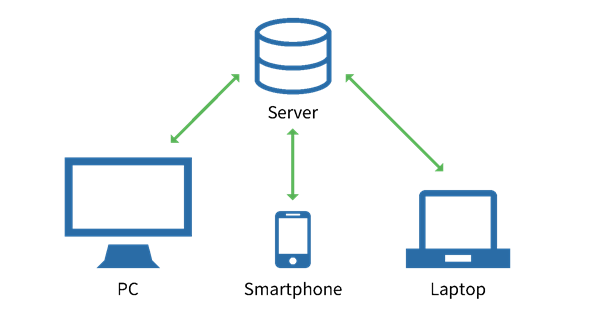
\includegraphics[width=1\textwidth]{images/ArchitecturalDesign/ClientServerModel.png}
        \caption{\label{fig:ClientServer}Client-Server architecture}
    \end{figure}
    
    The system is a distributed application which follows the well known client-server paradigm. It implements the thin-client technique, so as to facilitate supporting different client platforms. \par
    
    There are two main types of clients, the first will be the Web Application, and the second will be the Mobile Application. All the system business logic and data management will be contained and executed in the server.

    \begin{figure} [h]
        \centering
        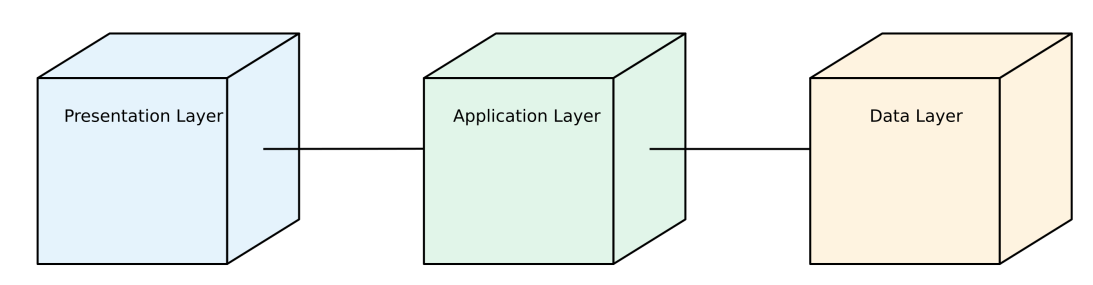
\includegraphics[width=1\textwidth]{images/ArchitecturalDesign/ThreeLayers.png}
        \caption{\label{fig:ThreeLayers}Three-Layers architecture}
    \end{figure}
    
    The system has three layers:
    \begin{itemize} 
        \item \textit{Presentation layer}: manages the presentation logic and the user interaction.
        \item \textit{Application layer}: manages the business logic and functions that the system must provide.
        \item \textit{Data layer}: manages the storage and retrieval of data.
    \end{itemize}
    
    These layers will be physically separated in the system, and will communicate through known APIs. \par

    \begin{figure} [h]
        \centering
        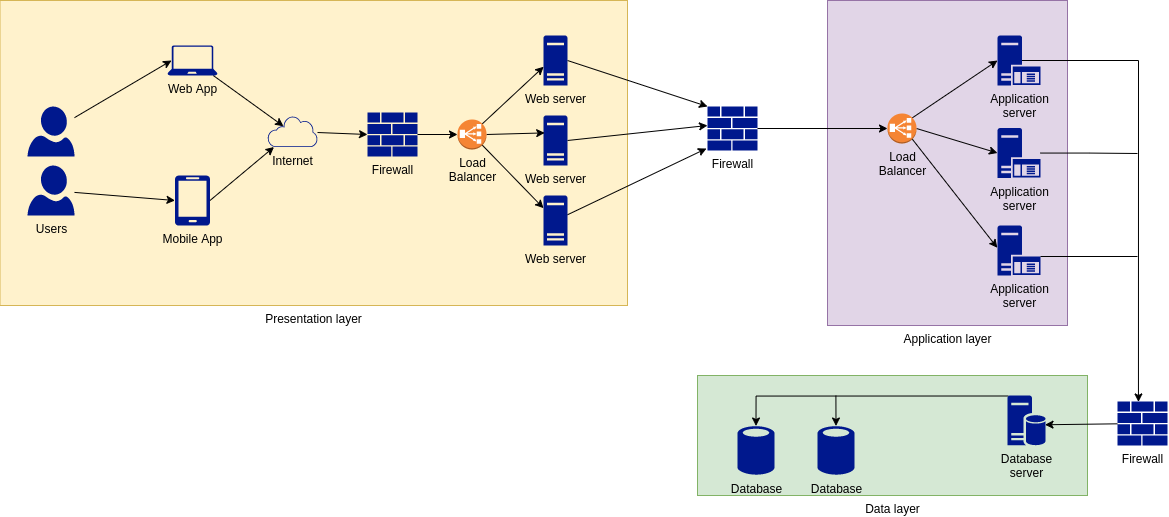
\includegraphics[width=1\textwidth]{images/ArchitecturalDesign/Architecture.png}
        \caption{\label{fig:Architecture}Architecture}
    \end{figure}
    
    \newpage

    The system also has four tiers:
    \begin{itemize}
        \item \textit{Client}: is either a web browser or a smartphone and will render the user interface.
        \item \textit{Web Server}: manages the incoming connections, prepares the user web pages and communicates requests to the application server.
        \item \textit{Application Server}: implements the business logic.
        \item \textit{Data Server}: implements the data storage and retrieval.
    \end{itemize}

    The first two tiers are used for the presentation layer, while the 3rd tier is for the application layer and the 4th tier is for the data layer. \par
    
    The client will communicate with the web servers, which will act as middleware and will interface with the application layer through its APIs. The application layer will then communicate to the data layer using the DBMS APIs. \par

    The application server APIs are RESTful, to better ease the portability of the client code and to guarantee flexibility for scaling. For communicating with the data layer, the ORM technique is used to exploit the object-oriented paradigm to also access the relational database. \par

    Every physical layer will be separated through a firewall and every communication will be encrypted using the HTTPS standard. \par

    The system component will now be described in more depth.
    

\newpage

\subsection{Component view}

    \begin{figure} [h]
        \centering
        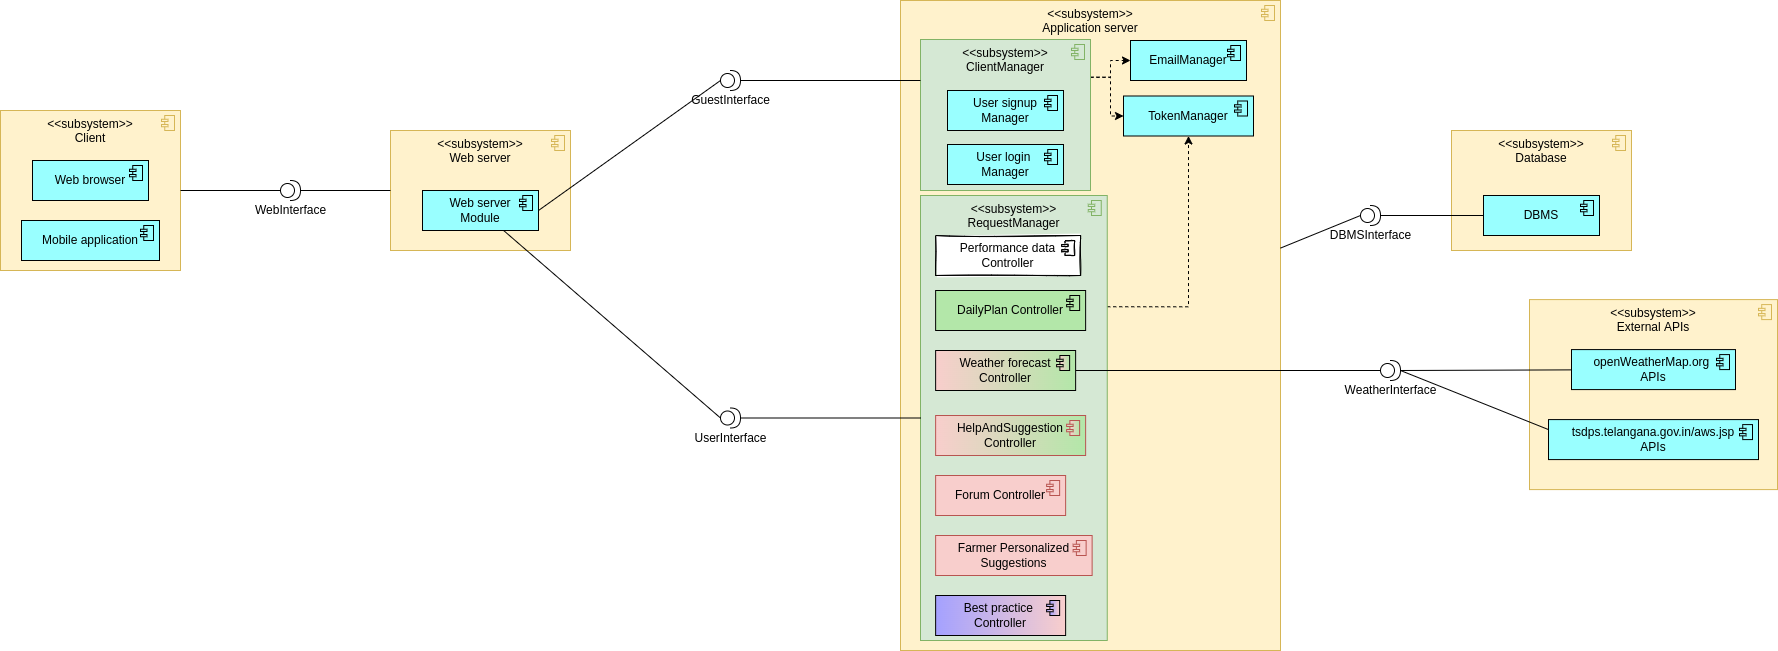
\includegraphics[width=1\textwidth]{images/ArchitecturalDesign/ComponentView.png}
        \caption{\label{fig:ComponentView}Component View}
    \end{figure}
    
    In the above figure we can see in more detail the components that are part of our system. \par
    
    \begin{itemize}
        \item \textbf{Web Server}: it has the function of routing requests from the clients to the application server and prepares part of the presentation.
        
        \item \textbf{Client manager}: it handles all the requests from unauthenticated users, giving them the possibilities of signup or authenticating them. It uses the login interface to manage all the requests and is capable of releasing authentication tokens that will be used for service with the other RESTful APIs. The token will also identify a request for its type of user, if it’s a farmer, agronomist or policy maker.
        
        \item \textbf{Request manager}: it checks a request token and route each request to the correct controller. Each controller has all the functions needed to support its feature. They are color coded to express which user type they must serve, green for agronomists, red for farmers, blue for policy makers and white for all three.
        
        \item \textbf{Email manager}: it handles the management of email, with built in components for scheduling or sending.
        
        \item \textbf{Token manager}: it manages, creates, checks and deletes authentication token, used for authenticating the REST requests.
        
        \item \textbf{DBMS}: it is the relational database controller that manages the storage and retrieval of data, but also the replication and security of such.
        
        \item \textbf{External APIs}: they represent the APIs of external services, for retrieving weather data.
        
    \end{itemize}
    

\newpage

\subsection{Deployment view}

    \begin{figure} [h]
        \centering
        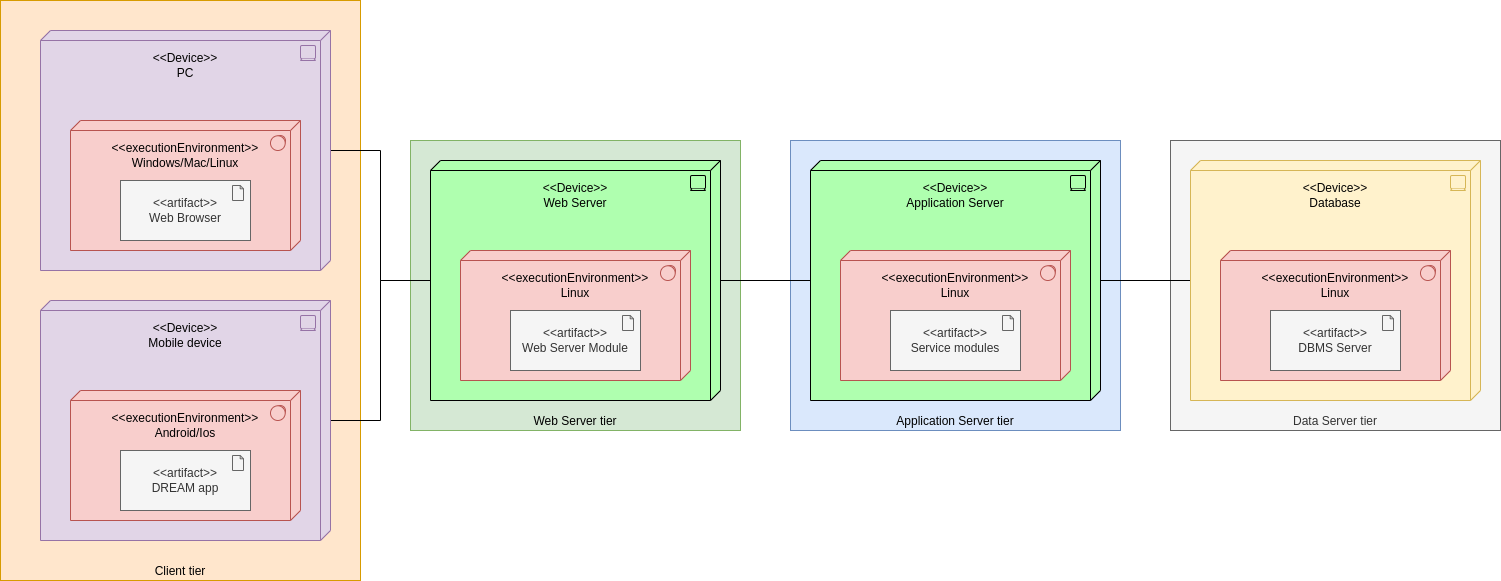
\includegraphics[width=1\textwidth]{images/ArchitecturalDesign/DeploymentView.png}
        \caption{\label{fig:DeploymentView}Deployment View}
    \end{figure}
    
    In the above figure is shown the deployment diagram, that shows the needed components for the system to run correctly. Each of these devices has its own operating system where software components run. Copies of these devices can be added to scale out the system. \par
    
    The tiers are four:
    \begin{itemize}
    
        \item \textbf{Client tier}: these are the client machines, which will run either a browser or the mobile application. To extend the audience the support will be to all major browsers (running on all major os) and mobile operating systems.
        
        \item \textbf{Web server tier}: this tier includes replicated web servers which receive requests from the clients and routes them to the API of the application server, preparing an HTML page to be rendered on the client, using also client-side scripting and style sheets.
        
        \item \textbf{Application server tier}: this tier contains replicated application servers which will serve the requests coming from the web servers. It implements all the business logic. To store and retrieve data it will communicate to the Data server tier through the DBMS interface.
        
        \item \textbf{Data server tier}: this tier includes the machine that will execute the DBMS and the data storage devices. It will execute the requests coming from the application server, storing data securely and with backups options.
        
    \end{itemize}
    

\newpage

\subsection{Runtime view}

    \subsubsection{User Sign Up}
        \begin{figure} [h]
            \centering
            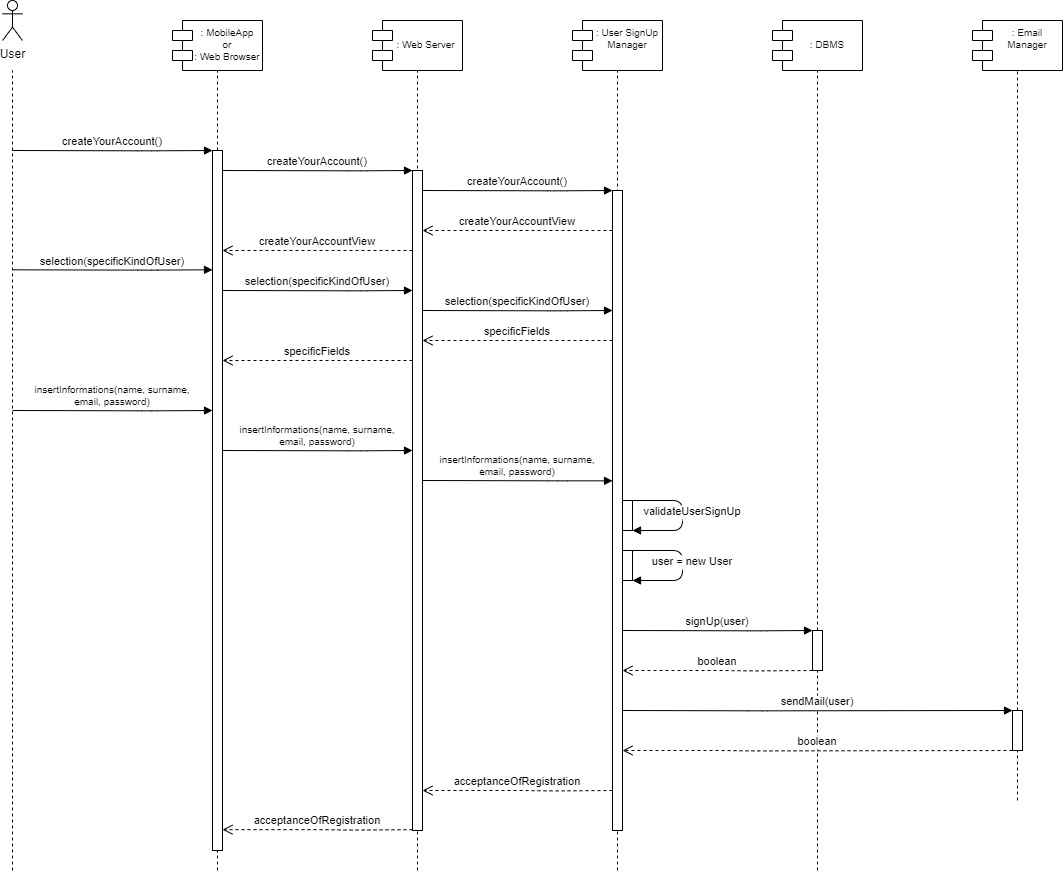
\includegraphics[width=1\textwidth]{images/ArchitecturalDesign/RuntimeView/1. UserSignUp.jpg}
            \caption{\label{fig:userSignUp}User Sign Up}
        \end{figure}
        
        The diagram above represents the process of signing up a user (Farmer, Agronomist, or Policy Maker). \par 
        The three cases are considered together in order to avoid useless repetitions, since the only things that changes are the "specific fields" requested by the system to the user (which are the information inserted lately by the user), according to the selection made by the user itself between the three possible alternatives presented in "createYourAccountView", which are: Farmer, Agronomist, and Policy Maker. \par
        
        \begin{itemize}
            \item If the user is a \textit{Farmer}, the specific fields are: name, surname, email, password, farm's name, farm's location.
            \item If the user is an \textit{Agronomist}, the specific fields are: name, surname, email, password, responsible area. 
            \item If the user is an \textit{Policy Maker}, the specific fields are: name, surname, email, password.
        \end{itemize}


    \newpage

    
    \subsubsection{User Login}
        \begin{figure} [h]
            \centering
            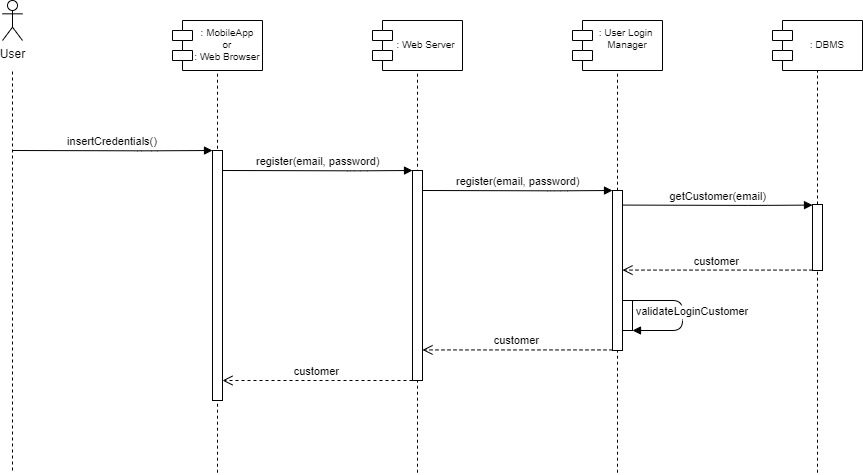
\includegraphics[width=1\textwidth]{images/ArchitecturalDesign/RuntimeView/2. UserLogin.jpg}
            \caption{\label{fig:userLogin}User Login}
        \end{figure}
        
        The diagram above represents the process of login of a user, who can be a Farmer, or an Agronomist, or a Policy Maker. \par 
        The user inserts his credentials (email and password), the systems checks if the credentials are correct and then shows the home page according to the user type.
        
    
    \newpage
    
    
    \subsubsection{Farmer visualize personalized suggestions}
        \begin{figure} [h]
            \centering
            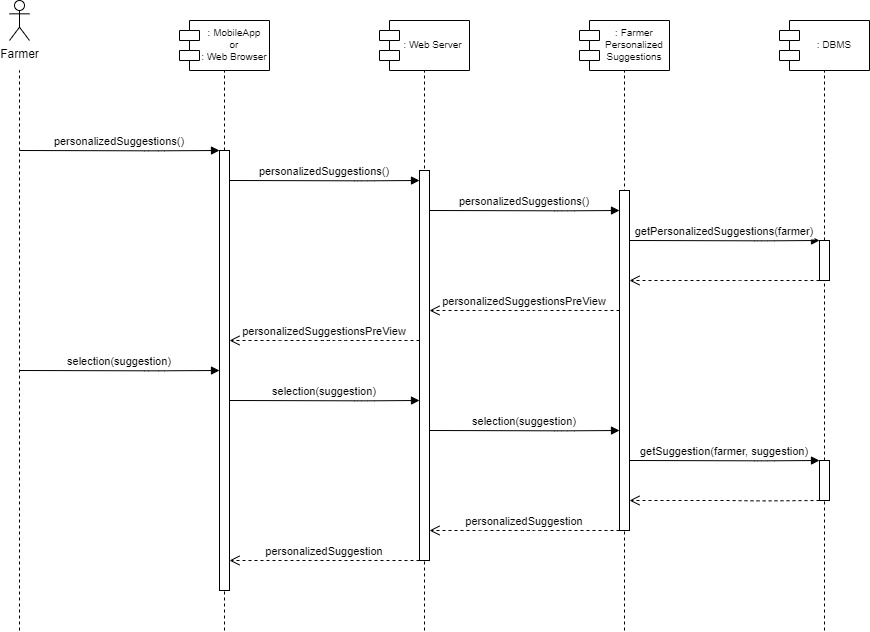
\includegraphics[width=1\textwidth]{images/ArchitecturalDesign/RuntimeView/3. FarmerVisualizePersonalizedSuggestions.jpg}
            \caption{\label{fig:farmerPersonalizedSuggestions}Farmer visualize personalized suggestions}
        \end{figure}
        
        The diagram above represents the process of viewing the personalized suggestions of a farmer, who is already on his home page. \par
        The system displays a preview of all the suggestions, then the farmer selects a specific suggestions through the ones showed, thus the system displays the selected suggestion with all the particulars.
        
    
    \newpage
    
    
    \subsubsection{Farmer inserts production data}
        \begin{figure} [h]
            \centering
            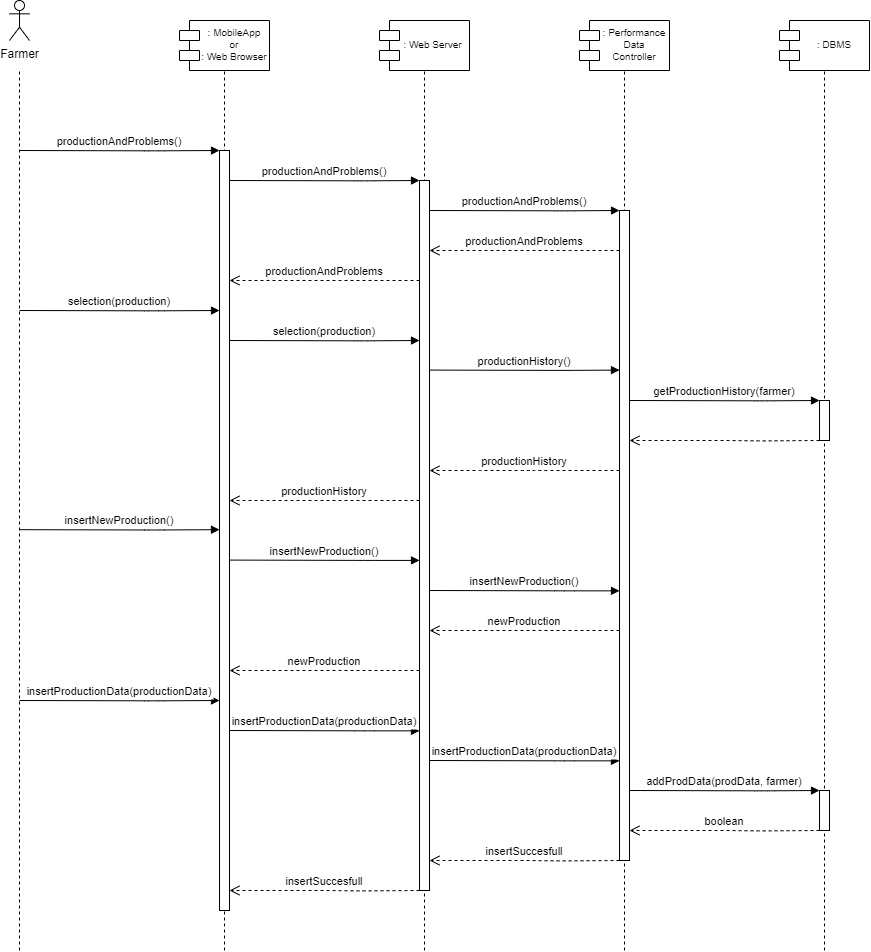
\includegraphics[width=1\textwidth]{images/ArchitecturalDesign/RuntimeView/4. FarmerInsertProductionData.jpg}
            \caption{\label{fig:farmerInsertsProductionData}Farmer inserts production data}
        \end{figure}
        
        The diagram above represents the process of inserting into the system the production data by a farmer, who is already on his home page. \par
        The system first asks between inserting production data and reporting a problem, and then, after the farmer selects to insert production data, displays the production data history of the farmer. \par
        The farmer is now able to click on the button "Insert Production Data", and after that the systems shows a list of fields that must be inserted by the farmer to correctly insert the production. \par
        The farmer inserts all the data, so that the system is able to store the production into the DB and, if everything works properly, displays a message saying that the data are stored. \par
        
    
    \newpage
    
    
    \subsubsection{Farmer reports a problem}
        \begin{figure} [h]
            \centering
            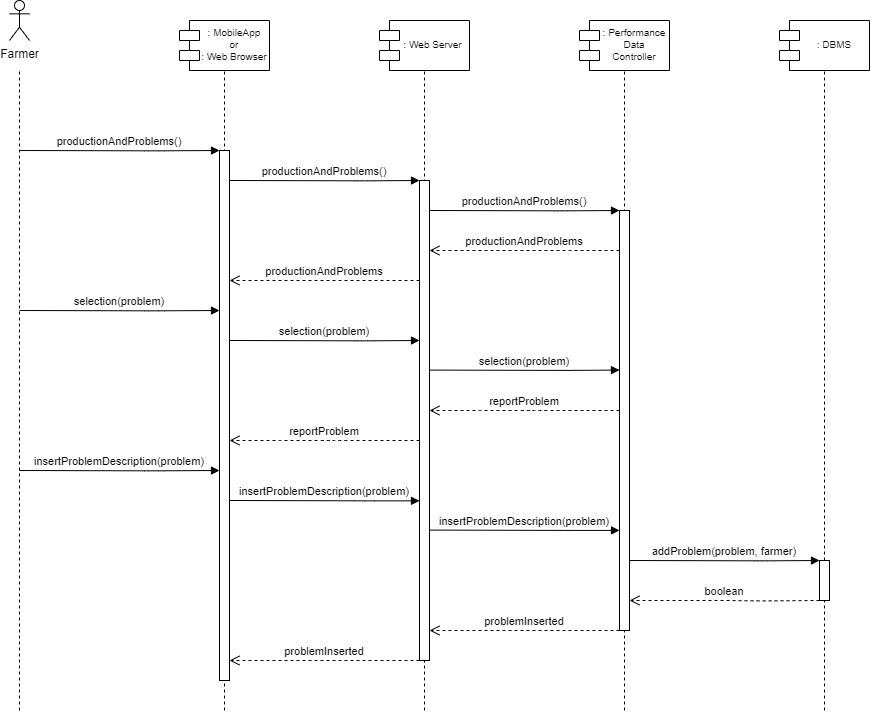
\includegraphics[width=1\textwidth]{images/ArchitecturalDesign/RuntimeView/5. FarmerReportAProblem.jpg}
            \caption{\label{fig:farmerReportProblem}Farmer reports a problem}
        \end{figure}
        
        The diagram above represents the process of reporting a problem by a farmer, who is already on his home page. \par
        The system first asks between inserting production data and reporting a problem, and then, after the farmer selects to report a problem, asks a description of the problem and shows the agronomists responsible of the farmer's area. \par
        The farmer can now insert the description of the problem and selects an agronomist to which request for help. \par
        The system is able to store the problem into the DB and, if everything works properly, displays a message saying that the problem is stored and then the farmer home page. \par
        
    
    \newpage
    
    
    \subsubsection{Farmer requests for help and suggestions}
        \begin{figure} [h]
            \centering
            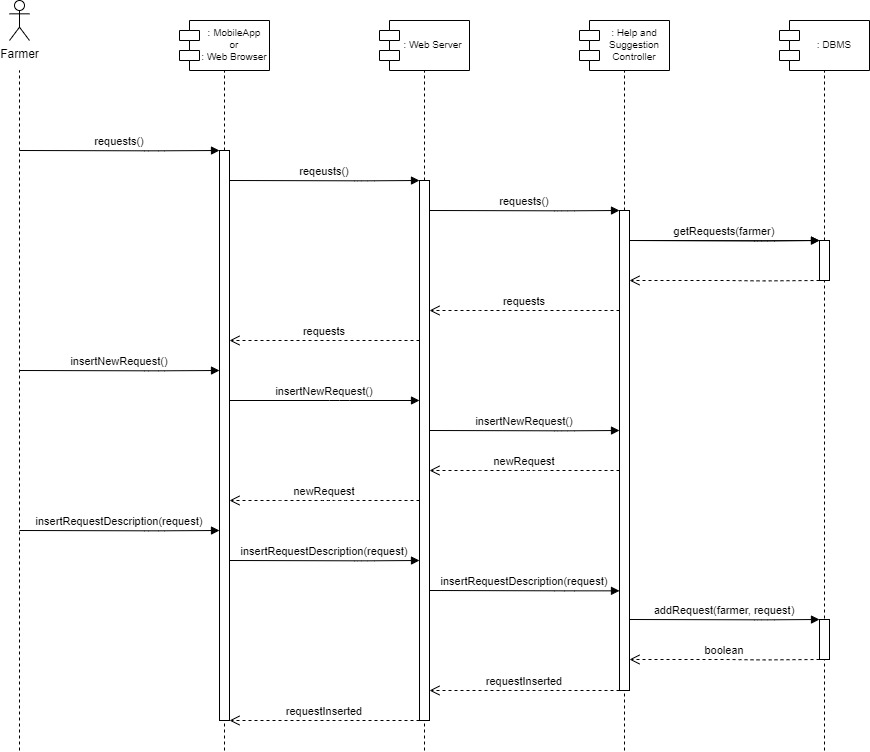
\includegraphics[width=1\textwidth]{images/ArchitecturalDesign/RuntimeView/6. FarmerRequestHelp.jpg}
            \caption{\label{fig:farmerRequestHelp}Farmer requests help}
        \end{figure}
        
        The diagram above represents the process of requesting help by a farmer, who is already on his home page. \par
        The system first displays a list of the most recent received, and then, after the farmer selects to make a new request, asks a description of the problem and a preferred receiver (receiver can be either a farmer or an agronomist). \par
        The farmer can now insert the description of the problem and can selects a farmer or an agronomist to which request for help. \par
        The system is able to store the problem into the DB, to contact the selected receiver and, if everything works properly, to display a message saying that the request for help is sent. \par
    
    
    \newpage
    
    
    \subsubsection{Farmer writes a new post on a forum}
        \begin{figure} [h]
            \centering
            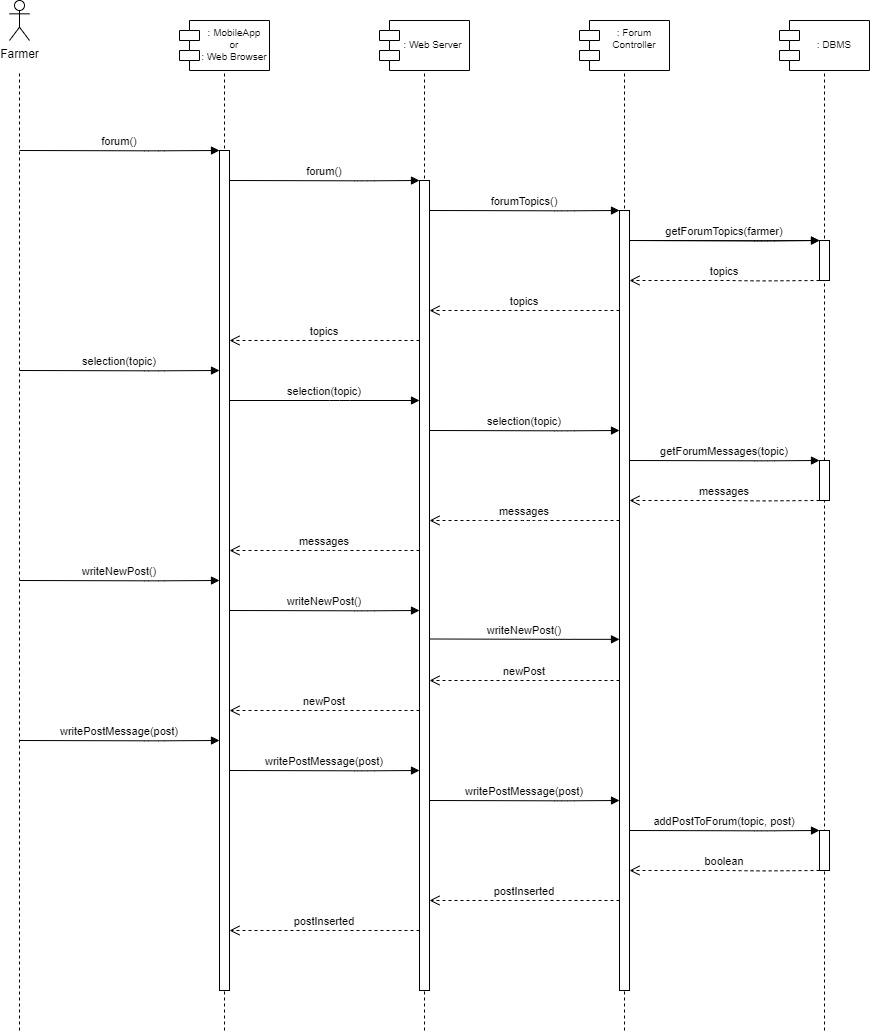
\includegraphics[width=0.9\textwidth]{images/ArchitecturalDesign/RuntimeView/7. FarmerWritesNewForumPost.jpg}
            \caption{\label{fig:farmerRequestHelp}Farmer requests help}
        \end{figure}
        
        The diagram above represents the process of writing a new post on the forum by a farmer, who is already on his home page. \par
        The system first displays a list of all the topics of the forum, and then, after the farmer selects a specific topic, shows the latest messages of the selected topic. \par
        The farmer clicks on the new post button, and then he can write the message; the system store the message into the DB and, if everything works properly, displays a message saying that the post has been created. \par
        
    
    \newpage
    
    
    \subsubsection{Farmer subscribes to a forum's topic}
        \begin{figure} [h]
            \centering
            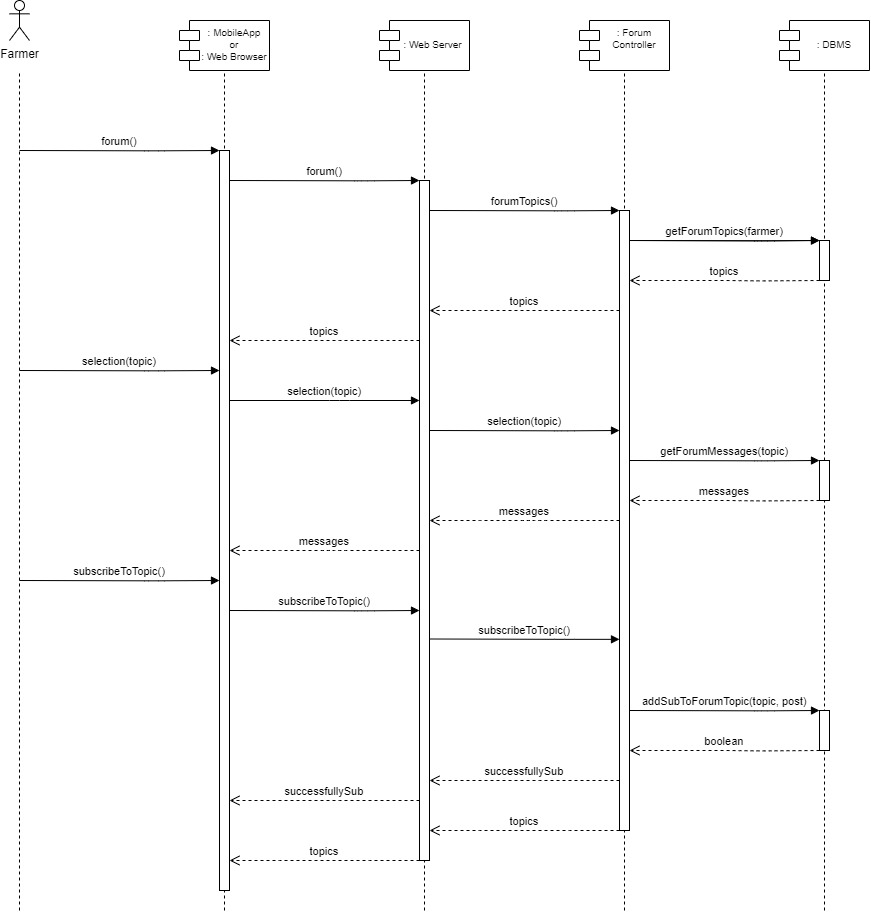
\includegraphics[width=1\textwidth]{images/ArchitecturalDesign/RuntimeView/8. FarmerSubscribeForumTopic.jpg}
            \caption{\label{fig:farmerSubscribeTopic}Farmer subscribes to a forum's topic}
        \end{figure}
        
        The diagram above represents the process of subscribing to a topic in the forum by a farmer, who is already on his home page. \par
        The system first displays a list of all the topics of the forum, and then, after the farmer selects a specific topic, shows the latest messages of the selected topic. \par
        The farmer clicks on the subscribe button; the system store the subscription into the DB and, if everything works properly, displays a message saying that the subscription has been successful and then shows the latest messages related to the topic. \par
    
    
    \newpage
    
    
    \subsubsection{Agronomist visualizes a daily plan}
        \begin{figure} [h]
            \centering
            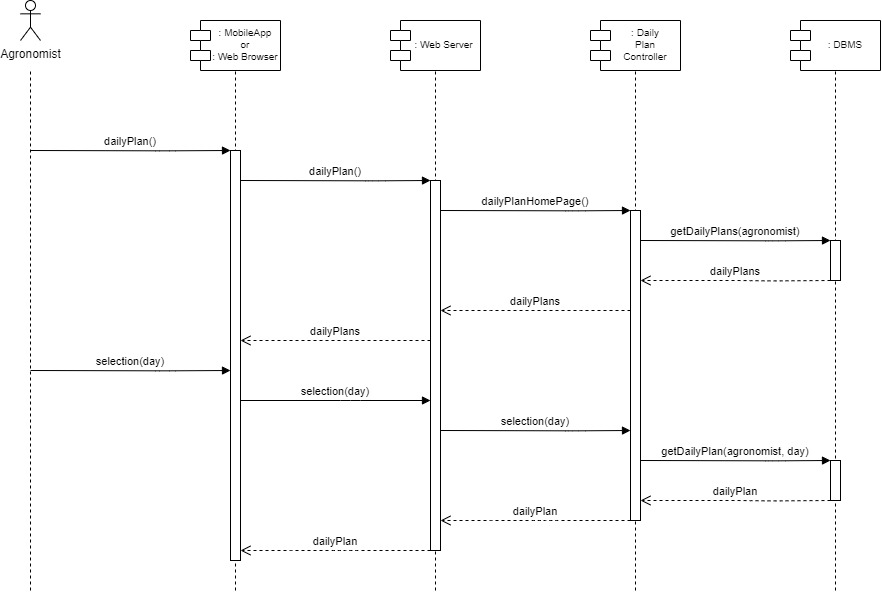
\includegraphics[width=1\textwidth]{images/ArchitecturalDesign/RuntimeView/9. AgronomistVisualizeDailyPlan.jpg}
            \caption{\label{fig:agronomistVisualizeDailyPlan}Agronomist visualizes a daily plan}
        \end{figure}
        
        The diagram above represents the process of viewing a daily plan (already inserted) by an agronomist, who is already on his home page. \par
        The system first displays a month calendar with, and then, after the agronomist selects a specific day, shows the daily plan of the selected day. \par
        
    
    \newpage
    
    
    \subsubsection{Agronomist inserts a daily plan}
        \begin{figure} [h]
            \centering
            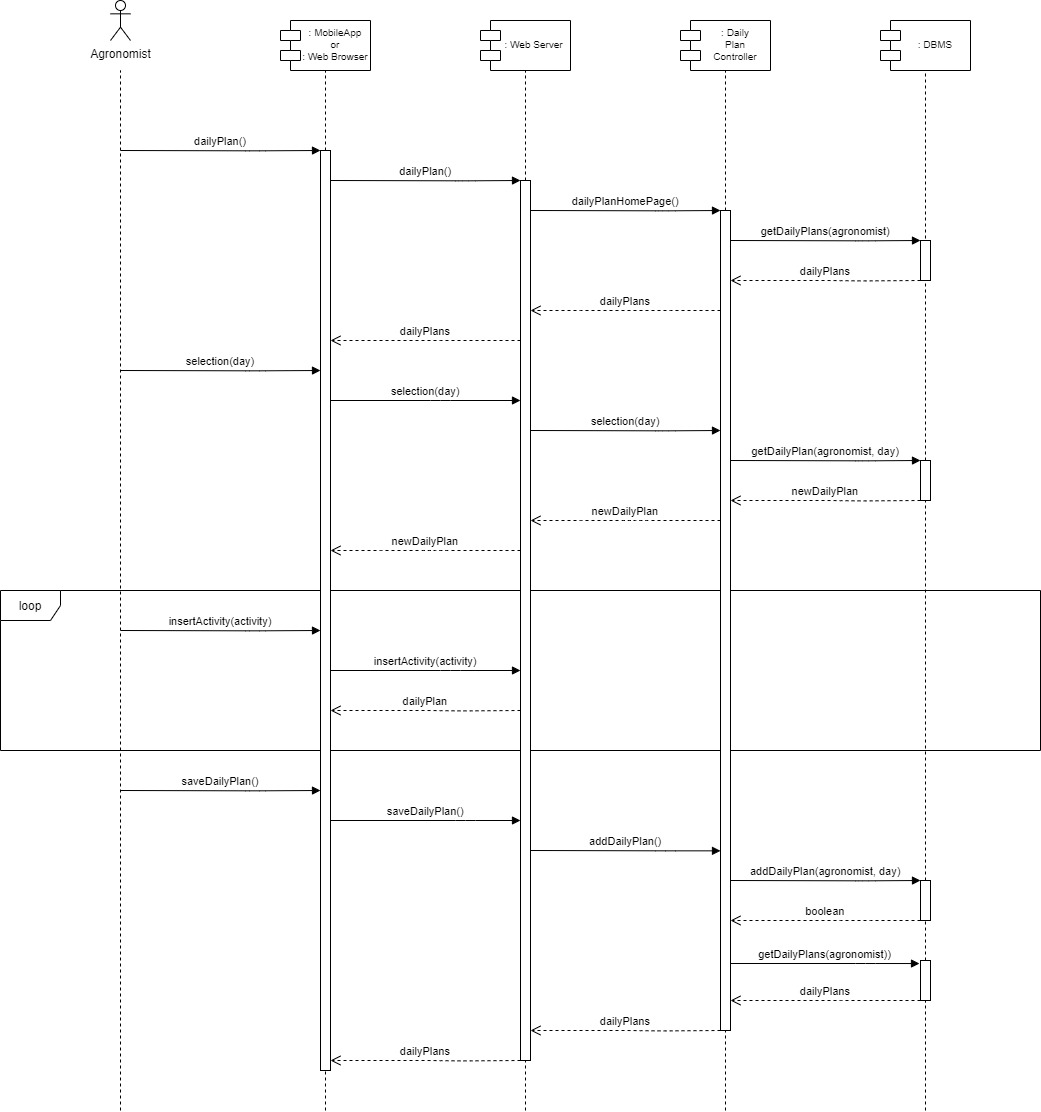
\includegraphics[width=1\textwidth]{images/ArchitecturalDesign/RuntimeView/10. AgronomistInsertDailyPlan.jpg}
            \caption{\label{fig:agronomistVisualizeDailyPlan}Agronomist visualizes a daily plan}
        \end{figure}
        
        The diagram above represents the process of inserting a daily plan by an agronomist, who is already on his home page. \par
        The system first displays a month calendar, and then, after the agronomist selects a specific day (with no daily plan inserted), allows the agronomist to recursively inserting new activity for the day. \par    
        When the agronomist clicks on save button, the system stores the new daily plan into the DB and, if everything works properly, displays a message saying that the daily plan has been successfully inserted and then shows again the calendar view. \par
        
        
    \newpage
    
    
    \subsubsection{Agronomist closes a daily plan}
        \begin{figure} [h]
            \centering
            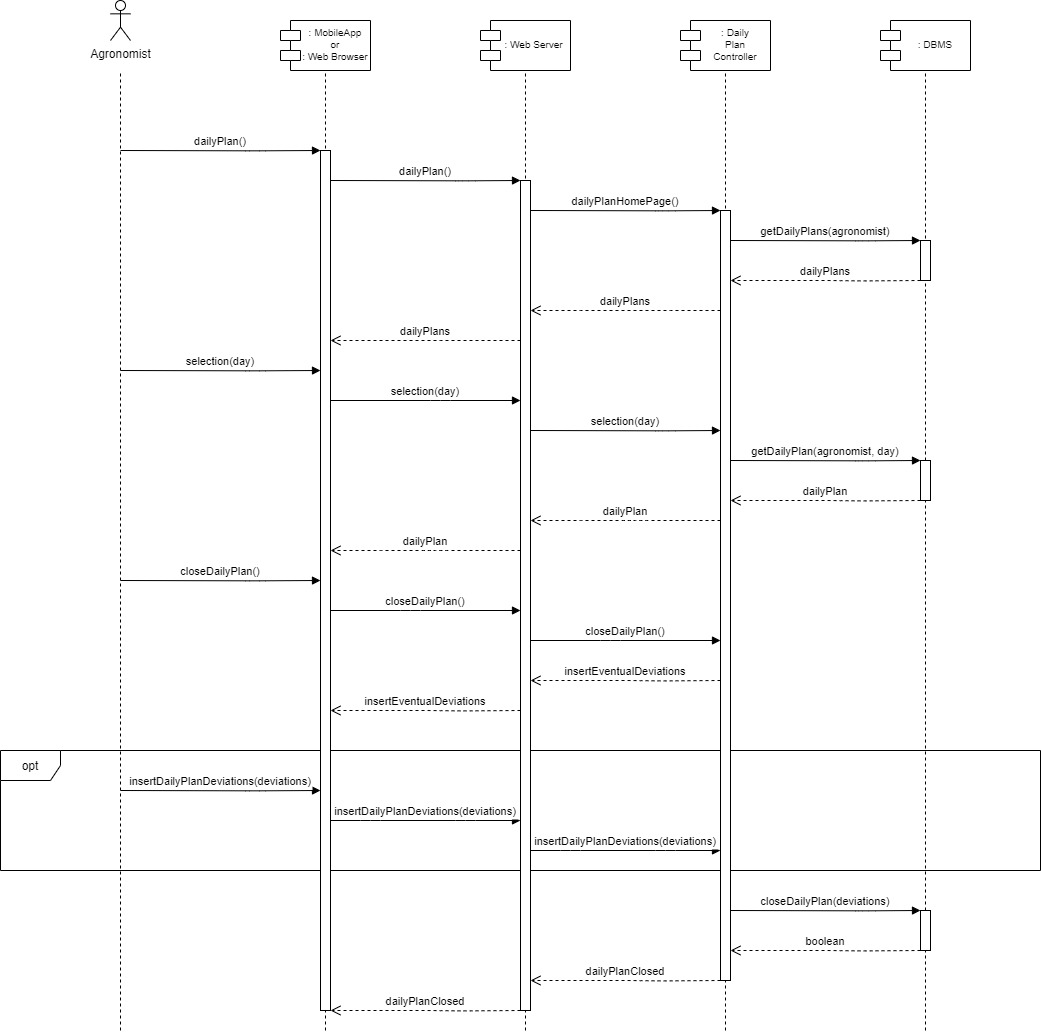
\includegraphics[width=1\textwidth]{images/ArchitecturalDesign/RuntimeView/11. AgronomistConfirmOrDeviationsOnDailyPlan.jpg}
            \caption{\label{fig:agronomistClosesDailyPlan}Agronomist confirms the execution of a daily plan (specifying eventually deviations)}
        \end{figure}
        
        The diagram above represents the process of closing a daily plan by an agronomist, who is already on his home page. \par
        The system first displays a month calendar, then, after the agronomist selects a specific day (with a daily plan inserted), shows the daily plan of the selected day. \par    
        When the agronomist clicks on confirm and specify deviations button, the system allows to insert optionally some deviations; the agronomist can just click on the confirm button, or can first insert the deviations and then click on the button.
        The daily plan is closed into the DB and, if everything works properly, displays a message saying that the daily plan has been successfully closed and then shows the agronomist home page. \par
    
    
    \newpage
    
    
    \subsubsection{Policy Maker visualizes farmers' production data}
        \begin{figure} [h]
            \centering
            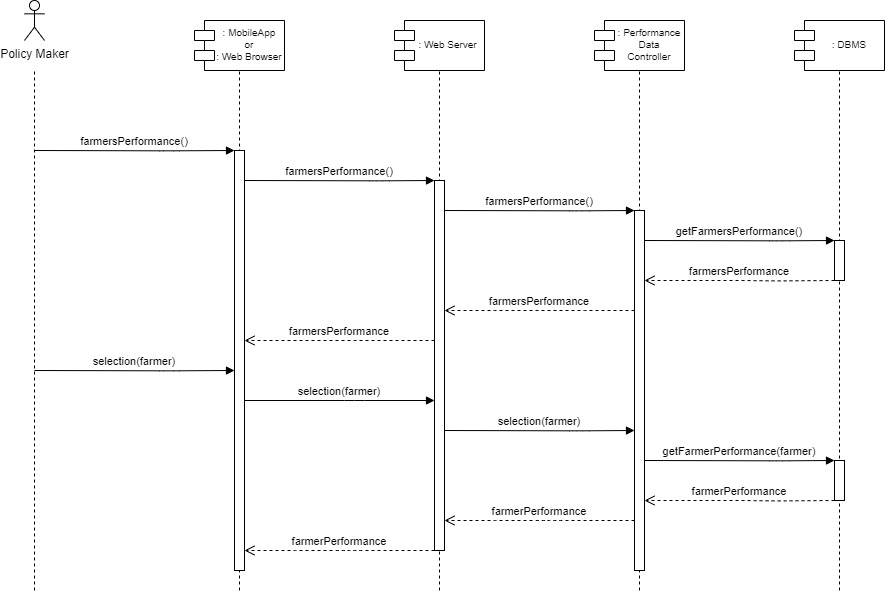
\includegraphics[width=1\textwidth]{images/ArchitecturalDesign/RuntimeView/12. PolicyMakerVisualizeProductionData.jpg}
            \caption{\label{fig:policyMakerVisualizeProdData}Policy Maker visualizes farmers' production data}
        \end{figure}
        
        The diagram above represents the process of visualizing the production data of farmers by a policy maker, who is already on his home page. \par
        The system first displays a graph with the overall results of the year and a list of farmers ordered by increasing performance, then, after the policy maker clicks on a specific farmer (one on top of the list), shows the production data about the farmer (corn produced, energy, fertilizer, and water used per unit). \par
        
        
    \newpage 
    
    
    \subsubsection{Policy Maker asks for best practices}
        \begin{figure} [h]
            \centering
            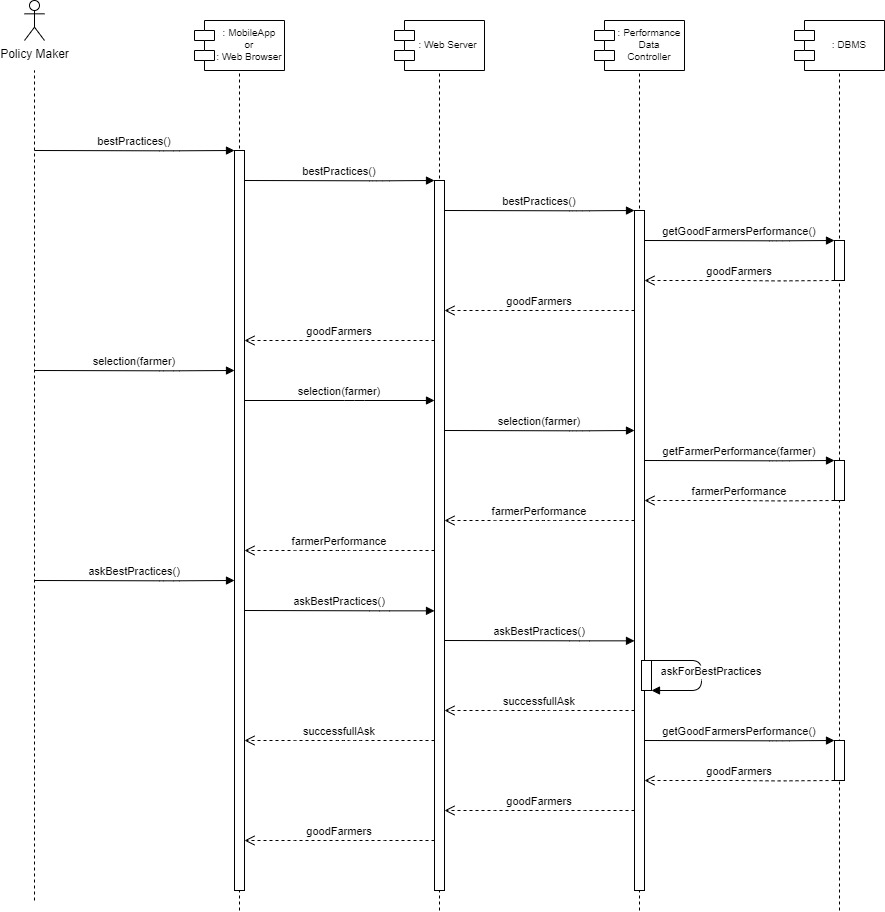
\includegraphics[width=1\textwidth]{images/ArchitecturalDesign/RuntimeView/13. PolicyMakerAskBestPractice.jpg}
            \caption{\label{fig:policyMakerAskBestPractice}Policy Maker asks for best practice}
        \end{figure}
        
        The diagram above represents the process of visualizing the production data of farmers by a policy maker, who is already on his home page. \par
        The system first displays a graph with the overall results of the year and a list of farmers ordered by increasing performance, then, after the policy maker clicks on a specific farmer (one on top of the list), shows the production data about the farmer. \par
        The policy maker clicks on ask for best practice button, and then the system shows a predefined message to be sent to the selected well performing farmer; when the policy maker clicks on send button, the system send the request to the farmer and shows again the list of farmers ordered by performance.
        
        
\newpage

\subsection{Component interfaces}

    \begin{figure} [h]
            \centering
            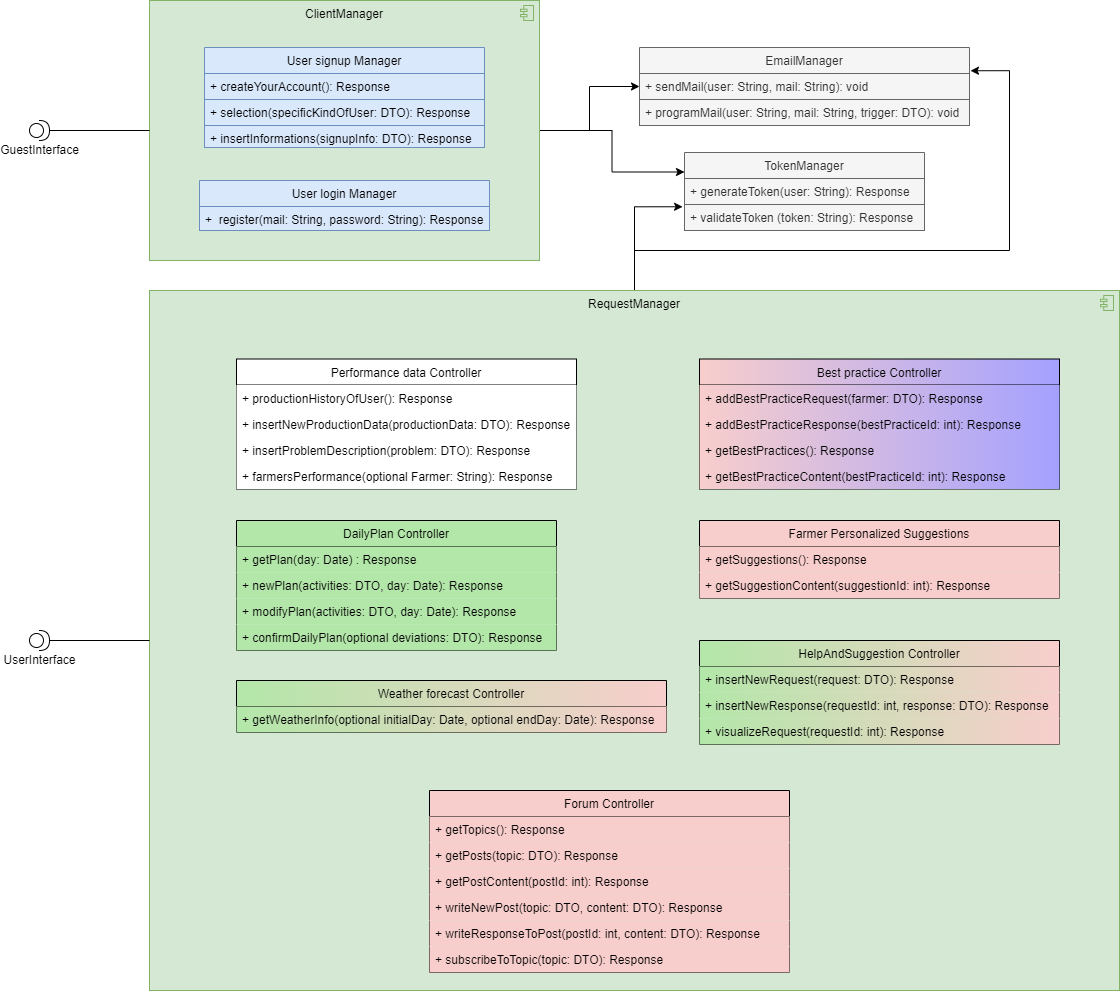
\includegraphics[width=1\textwidth]{images/ArchitecturalDesign/InterfaceView.png}
            \caption{\label{fig:InterfacesDiagram}Interfaces Diagram}
        \end{figure}

    The interfaces shown in the diagram are the essential one to support the Dream application. \par
    The Guest Interface is used for communication from unauthenticated users, while the User Interface is used for authenticated users communications. Every method through the User Interface will also carry the authentication token for securing the requests and recognising the user. \par


\newpage


\subsection{Architectural styles and patterns}

    \subsubsection{Four-tier system architecture}
    
    We chose this architecture mostly for portability: it decouples the client implementation from the business logic so it is easier to support a vast number of client types. \par
    A light client also means it can be supported on a vast variety of even older hardware. Other benefit from this choice are:
    
    \begin{itemize}
        \item \textit{Flexibility}: the communication through known interfaces makes the modification of single components easier without the need to check the entire system functionality.
        \item \textit{Scalability}: the separation of layers makes it easier to expand just the critical components, saving money and time on less critical parts of the system.
        \item \textit{Fault tolerance}: the presence of redundant servers guarantees functionality in the case of high load or some server fault.
        \item \textit{Load distribution}: the load balancer could be dynamically implemented to preview high spikes of load and dynamically assign and free computation power from the critical components. Especially useful if it is deployed in a server farm.
    \end{itemize}
    
    \subsubsection{RESTful architecture}

    The choice of the RESTful architecture to communicate to the application server brings many advantages:
    
    \begin{itemize}
        \item \textit{Scalability}, \textit{flexibility} and \textit{portability}: the stateless nature of the server leads to an easier maintenance, meaning that a server can be migrated or added without any changes to data.
        \item \textit{Independence}: the greater separation between the presentation and application layer makes the development of clients easier, so they can be built independently from the rest of the system.
    \end{itemize}
    
    \subsubsection{Model View Controller}
    
    Model-View-Controller is a design pattern used to divide the program into three interconnected elements. It is useful to separate the internal representation of information from how the information is then presented to the user. The three components are:

    \begin{itemize}
        \item \textit{Model}:the system internal dynamic data structure. It directly manages data and rules of the application. It keeps the internal state consistent.
        \item \textit{Controller}: accepts input from the view and applies elaboration to the model.
        \item \textit{View}: representation of the internal data for the user. Multiple views of the same information are possible.
    \end{itemize}
    


\newpage


\subsection{Other design decisions}

    \subsubsection{Thin Client}
    A thin client only has to display information on the screen. We chose this design for our system to be able to bring our application to the highest variety of devices possible. This eases the work of porting the application to new systems and guarantees that even low powered devices can run the application properly. The drawback of this choice is that we need to add the requirement for an internet connection.

    \subsubsection{Stateless components}
    The server components being stateless enables our system to be highly flexible and ease the work for scaling out, enabling the possibilities of an elastic load balancer to dynamically manage resources (and reduce costs). Adding new compute units is easy as they don’t need to copy or import any data, but they just need to execute the components. Also reliability of the system is increased as if a component fails no data will be lost and it can just be easily substituted.




\newpage

\newpage





\section{User Interface Design}

    \subsection{User}
    
    
    \begin{itemize}
        \item \textbf{Account creation}
    \end{itemize}
        \begin{figure} [h]
            \centering
            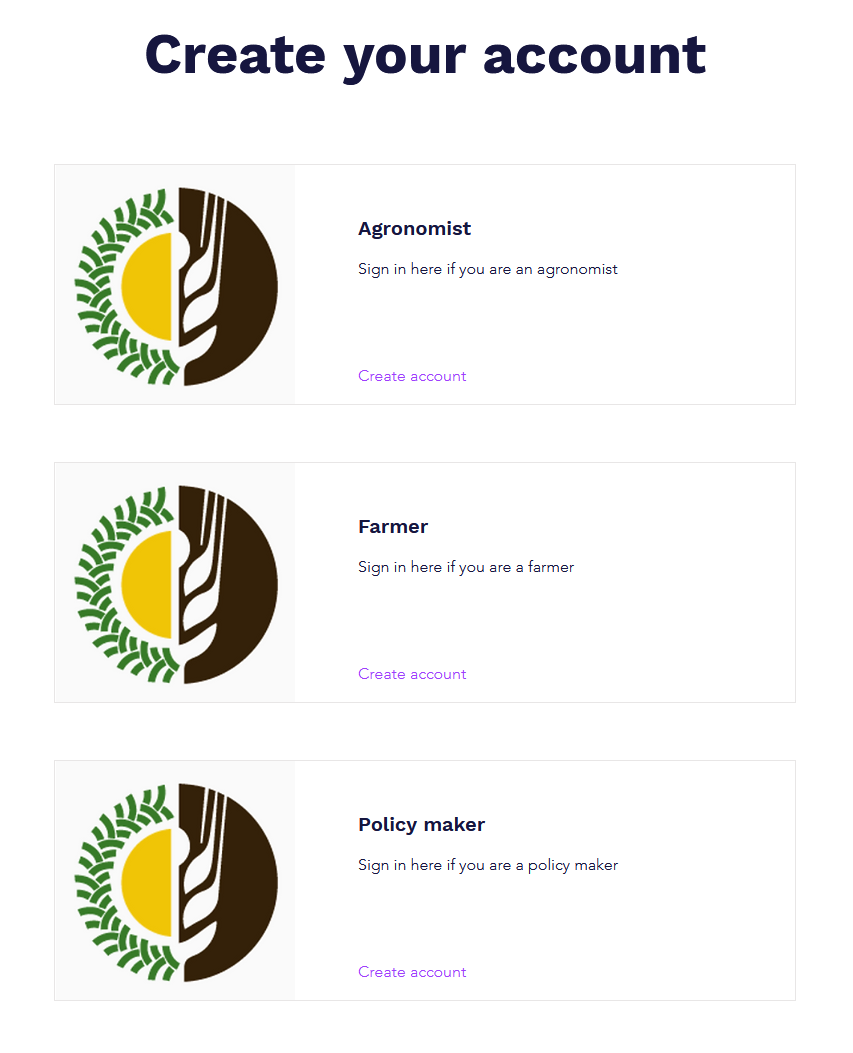
\includegraphics[width=0.7\textwidth]{images/UserInterfaces/CreateAccountWeb.png}
            \quad
            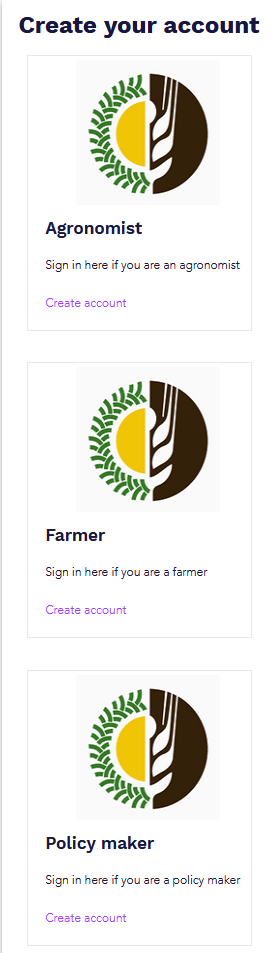
\includegraphics[width=0.2\textwidth]{images/UserInterfaces/CreateAccountApp.png}
            \quad
            \caption{\label{fig:accountCreation}Create Account; web on the left, app on the right}
        \end{figure}
    
    \newpage
    
    \begin{itemize}
        \item \textbf{First page after download}
    \end{itemize}
        \begin{figure} [h]
            \centering
            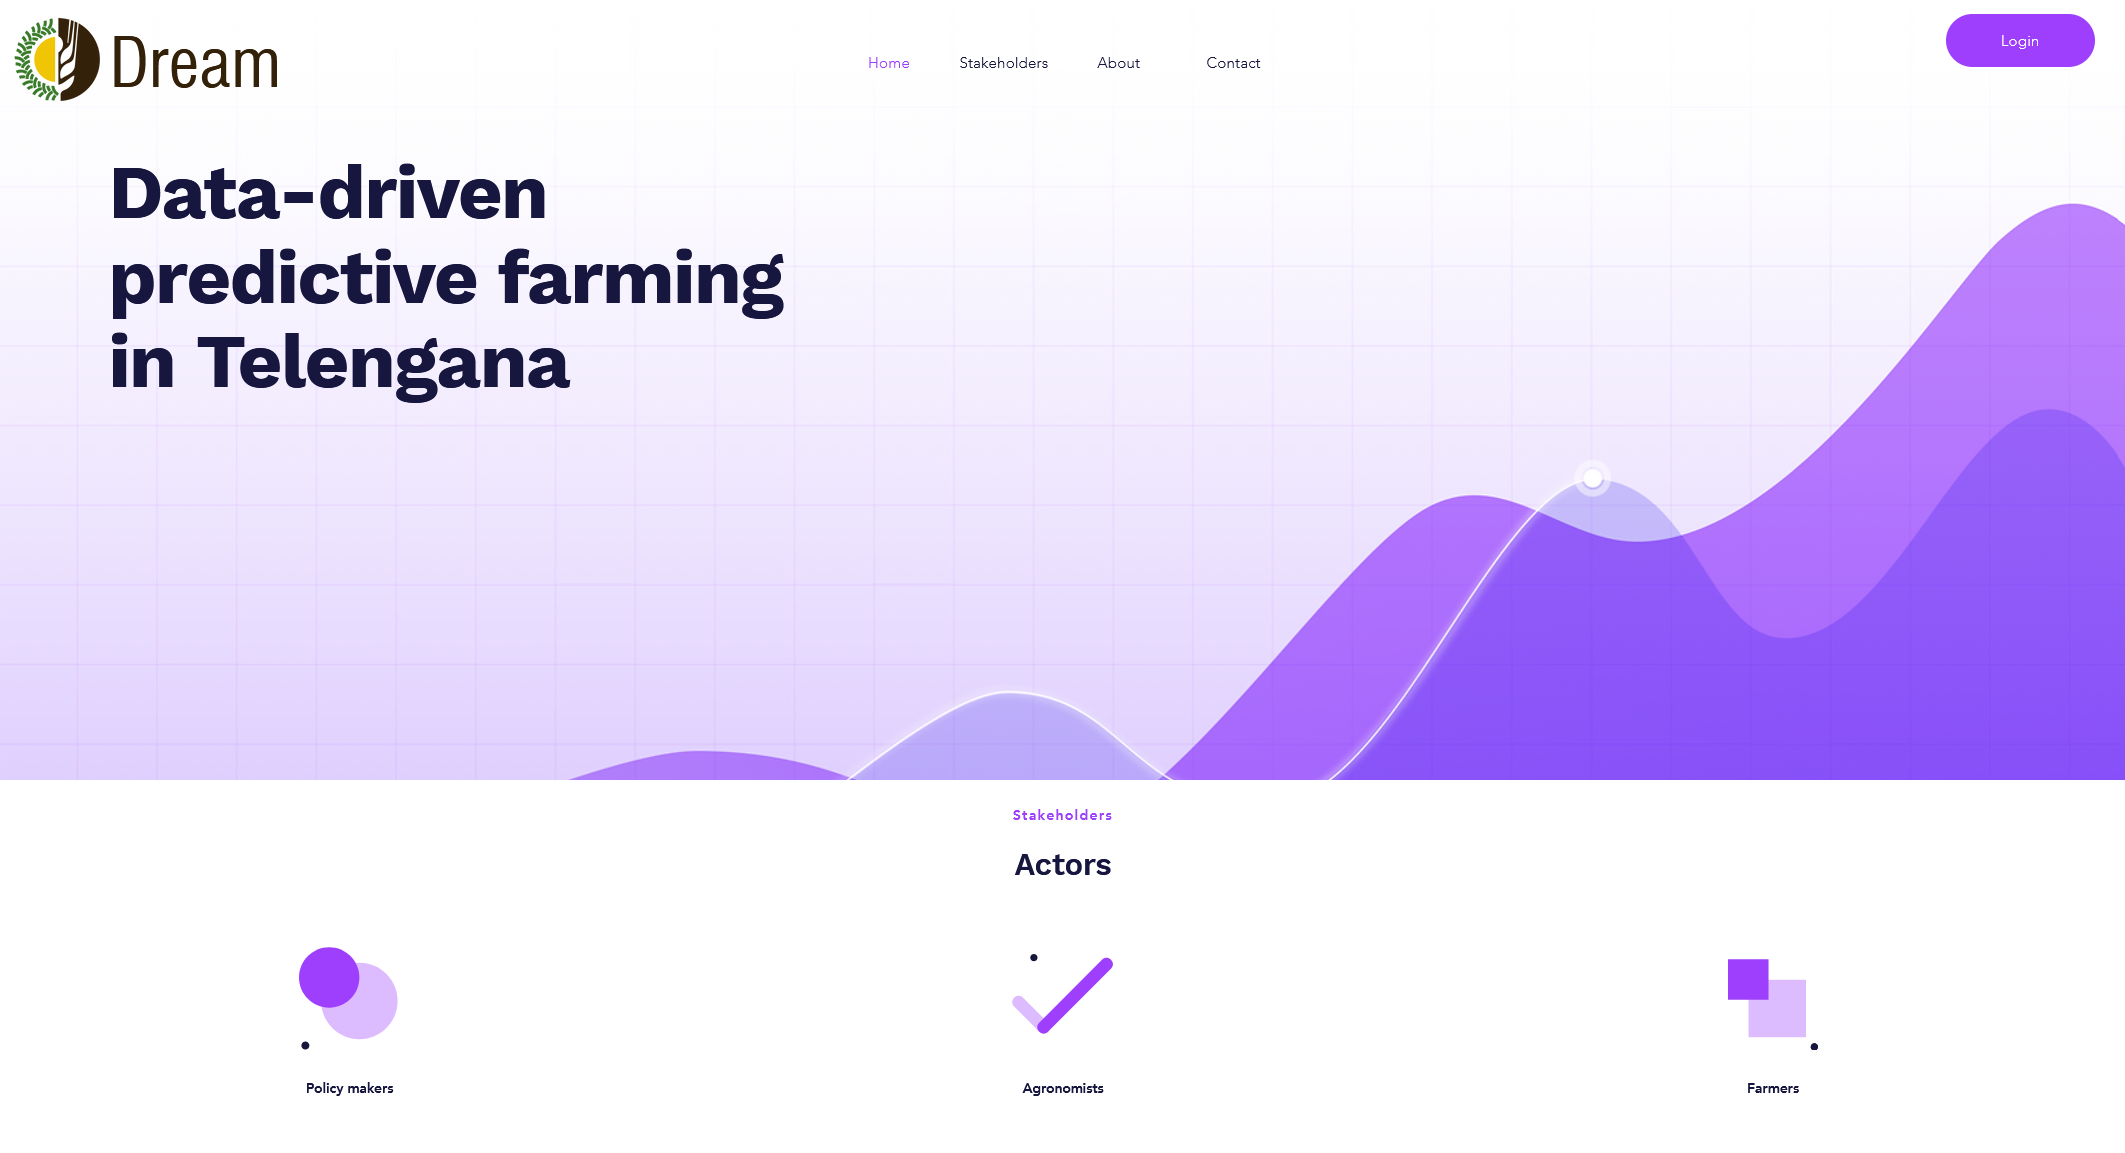
\includegraphics[width=0.7\textwidth]{images/UserInterfaces/FirstPageWeb.png}
            \quad
            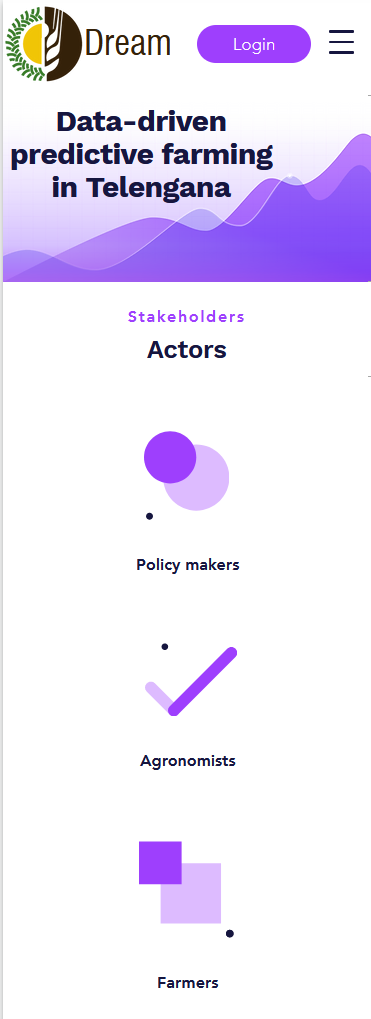
\includegraphics[width=0.2\textwidth]{images/UserInterfaces/FirstPageApp.png}
            \quad
            \caption{\label{fig:firstPage}First page; web on the left, app on the right}
        \end{figure}




    \begin{itemize}
        \item \textbf{User Login}
    \end{itemize}
        \begin{figure} [h]
            \centering
            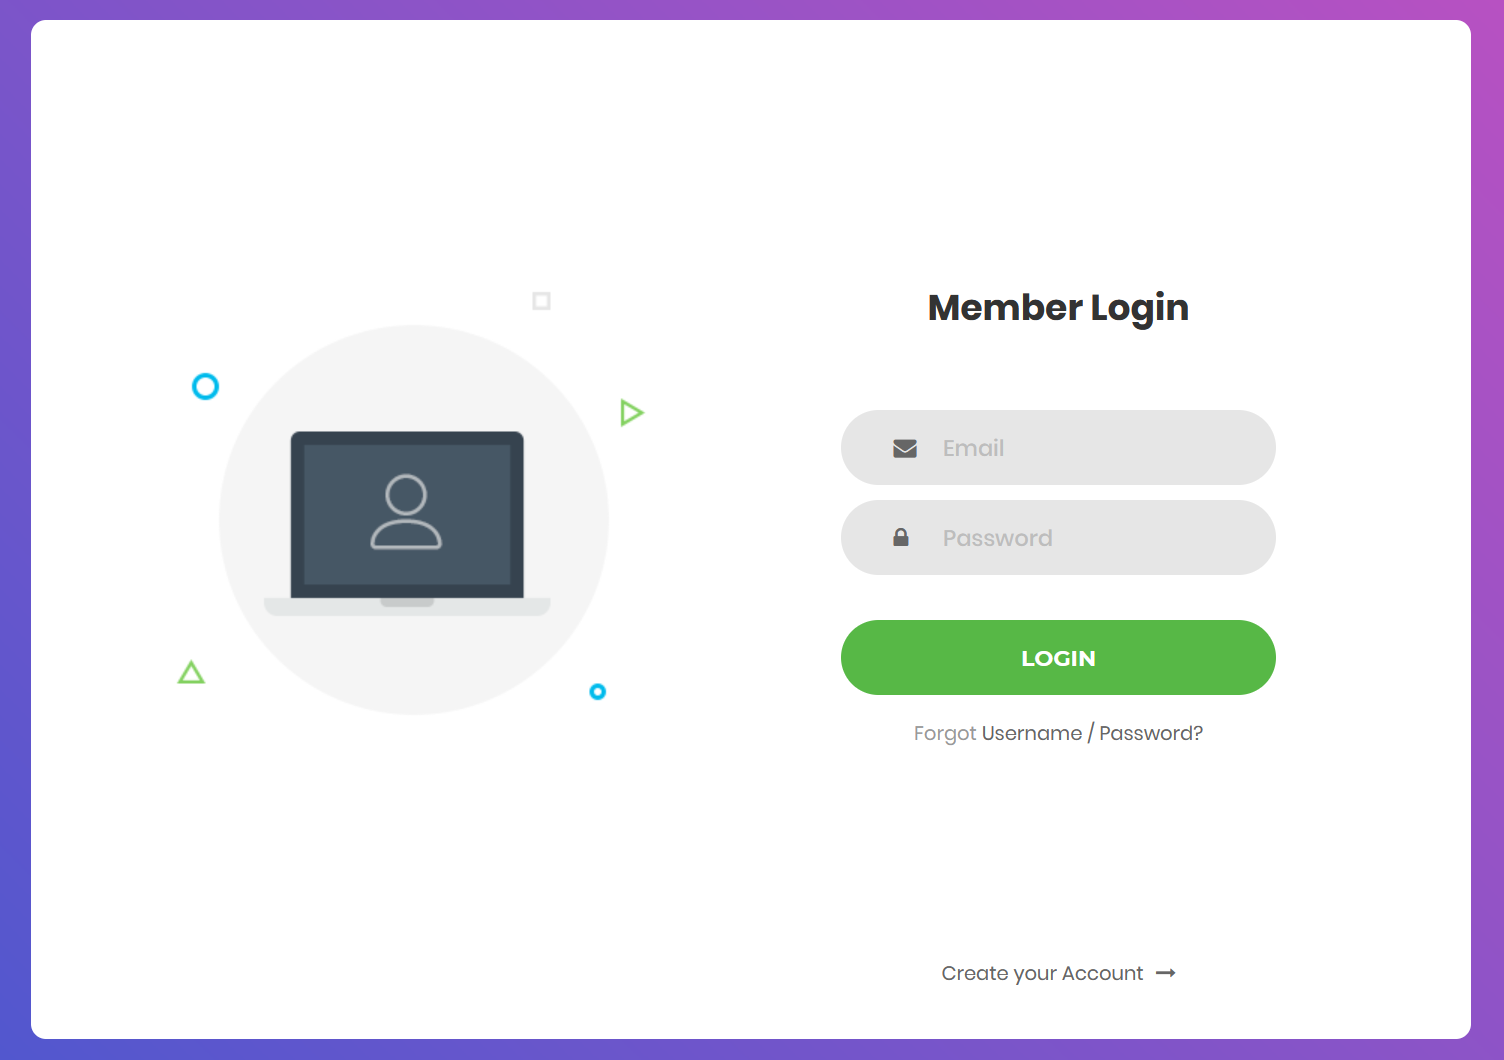
\includegraphics[width=0.5\textwidth]{images/UserInterfaces/UserLoginWeb.png}
            \quad
            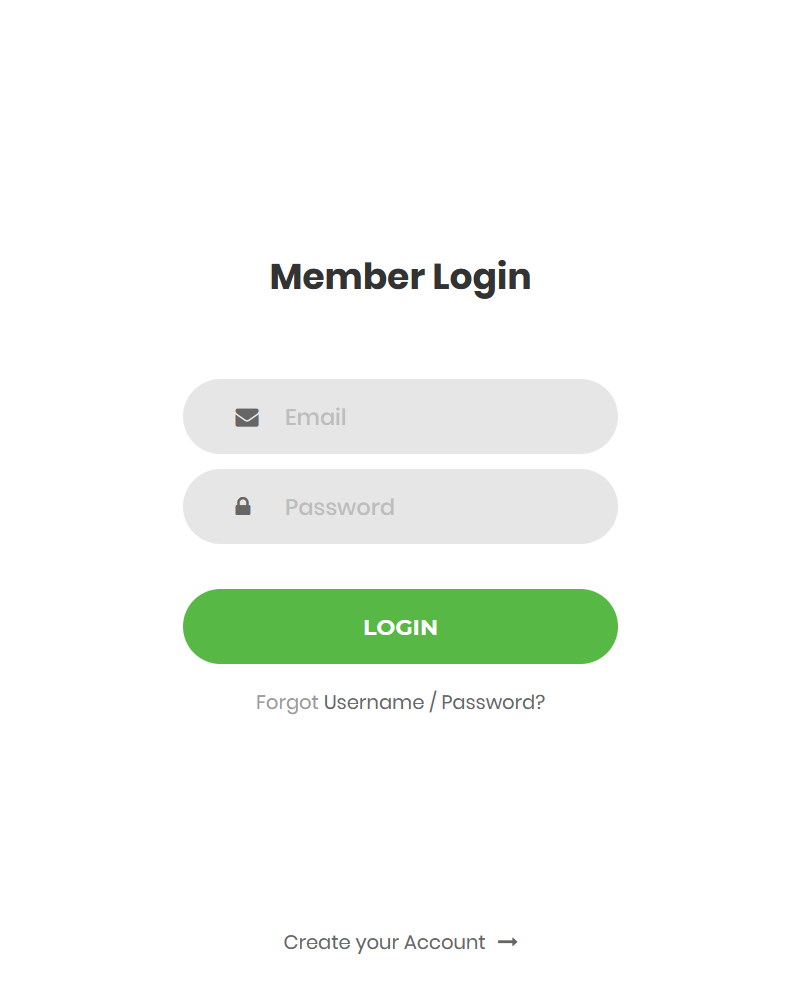
\includegraphics[width=0.3\textwidth]{images/UserInterfaces/UserLoginApp.png}
            \quad
            \caption{\label{fig:userLogin}User Login; web on the left, app on the right}
        \end{figure}
    
    
    \newpage
    
    
    \subsection{Farmer}
    
    \begin{itemize}
        \item \textbf{Farmer Sign In}
    \end{itemize}
        \begin{figure} [h]
            \centering
            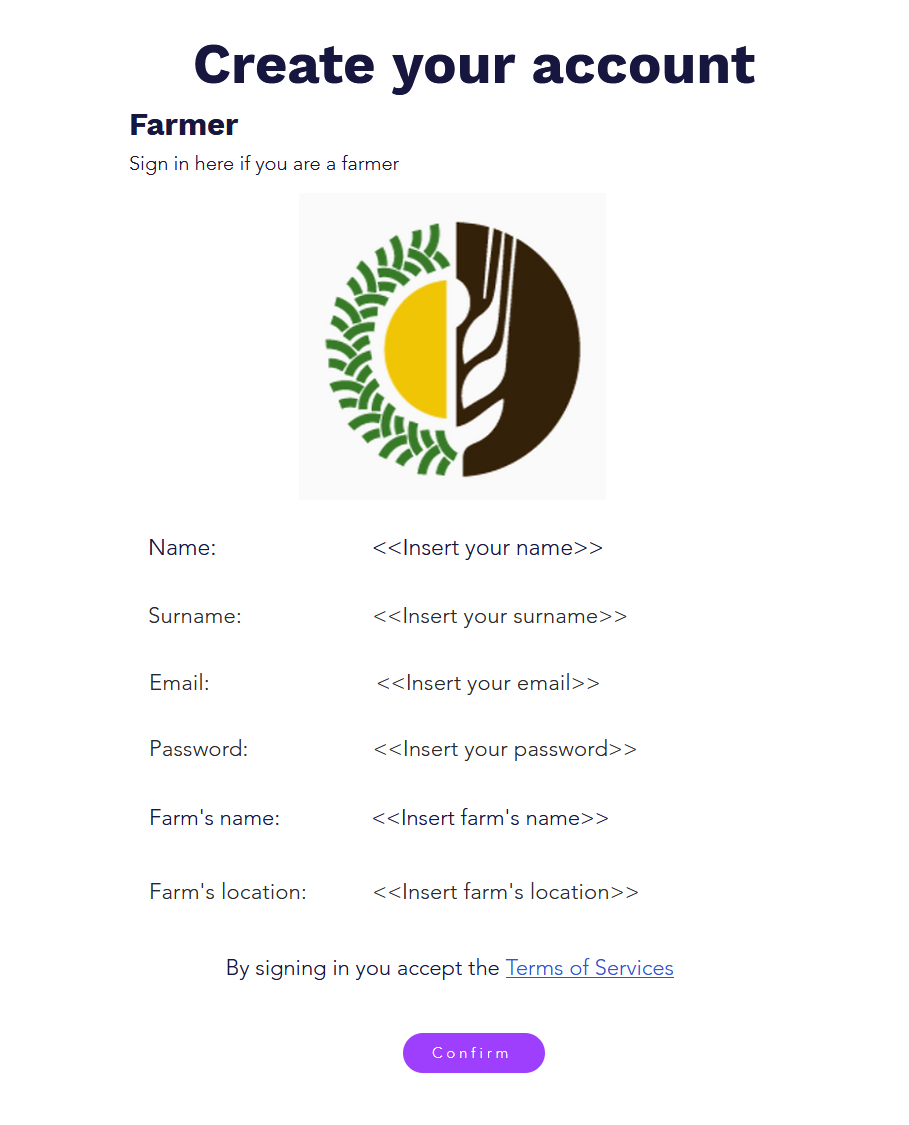
\includegraphics[width=0.7\textwidth]{images/UserInterfaces/Farmer/FarmerSignInWeb.png}
            \quad
            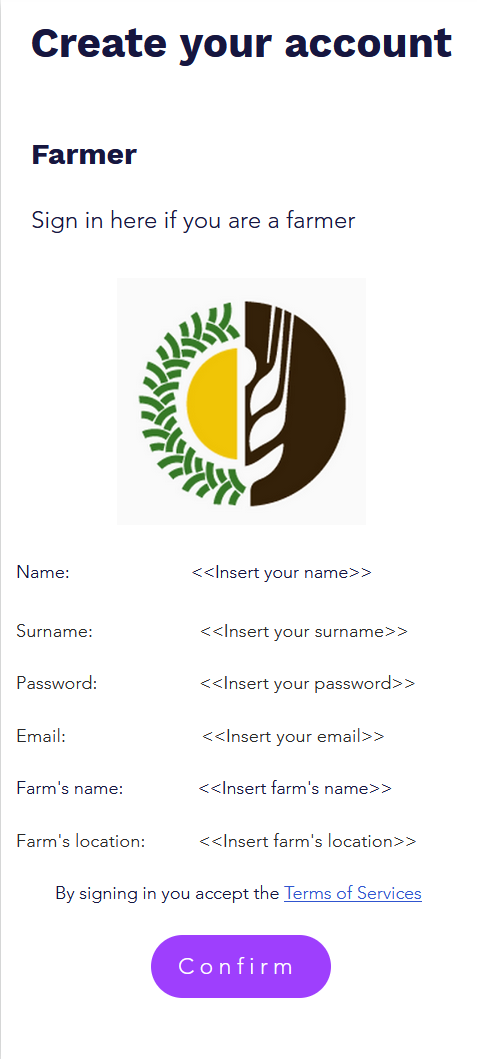
\includegraphics[width=0.2\textwidth]{images/UserInterfaces/Farmer/FarmerSignInApp.png}
            \quad
            \caption{\label{fig:farmerSignIn}Farmer Sign In; web on the left, app on the right}
        \end{figure}
    
    \newpage
    
    \begin{itemize}
        \item \textbf{Farmer Home Page}
    \end{itemize}
        \begin{figure} [h]
            \centering
            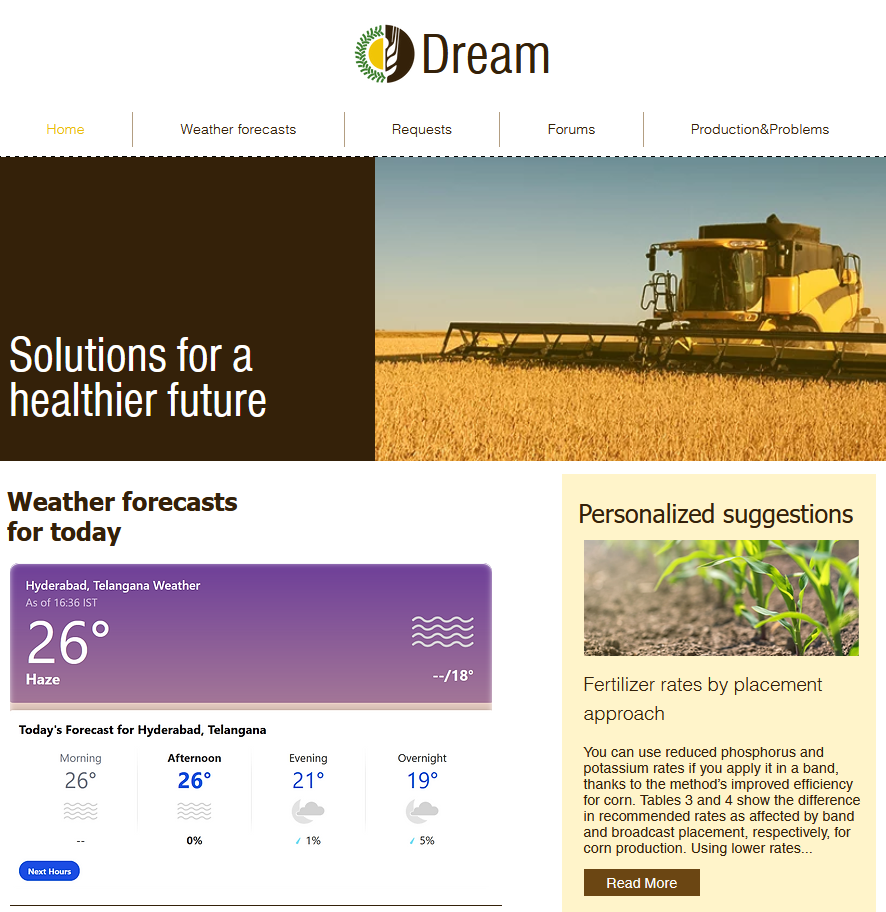
\includegraphics[width=0.7\textwidth]{images/UserInterfaces/Farmer/FarmerHomePageWeb.png}
            \quad
            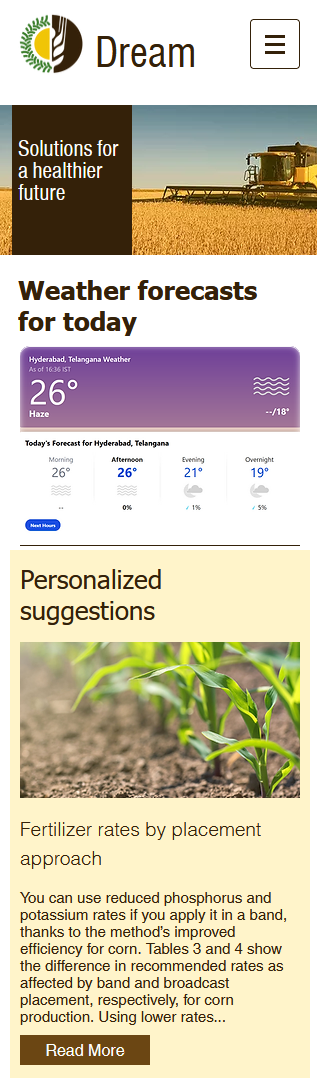
\includegraphics[width=0.2\textwidth]{images/UserInterfaces/Farmer/FarmerHomePageApp.png}
            \quad
            \caption{\label{fig:farmerHomePage}Farmer Home Page; web on the left, app on the right}
        \end{figure}
        
    \newpage
    
    \begin{itemize}
        \item \textbf{Farmer Best Practices}
    \end{itemize}
        \begin{figure} [h]
            \centering
            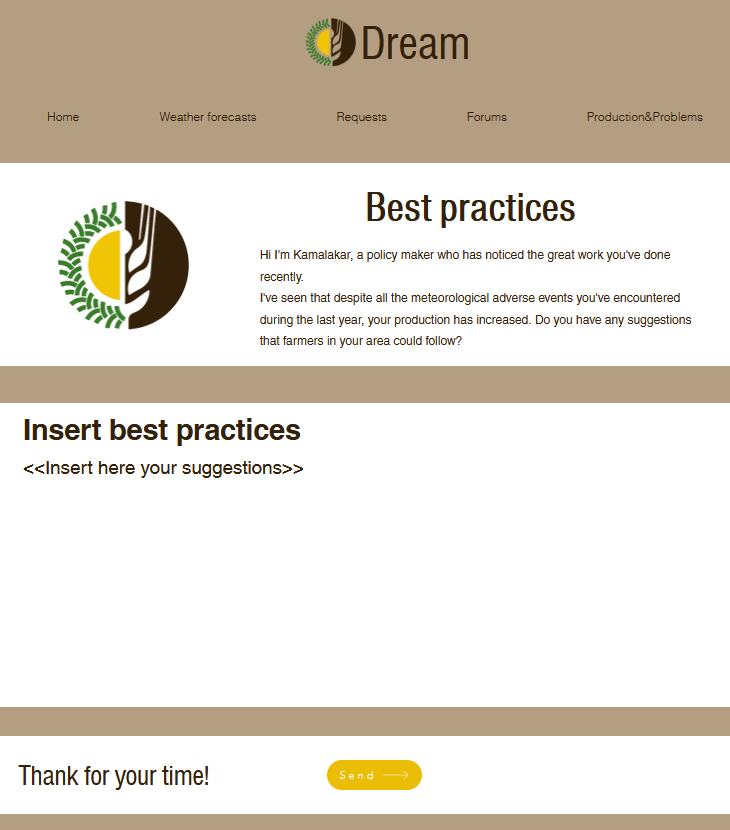
\includegraphics[width=0.7\textwidth]{images/UserInterfaces/Farmer/BestPractices/InsertBestPracticesWeb.png}
            \quad
            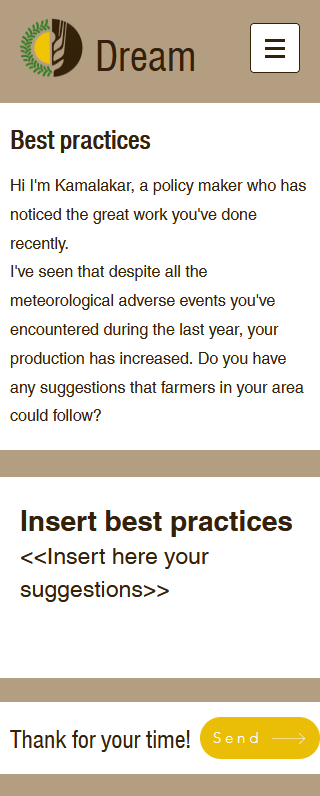
\includegraphics[width=0.2\textwidth]{images/UserInterfaces/Farmer/BestPractices/InsertBestPracticesApp.png}
            \quad
            \caption{\label{fig:farmerBestPractices}Farmer inserts Best Practices; web on the left, app on the right}
        \end{figure}
        
    \newpage
    
    \begin{itemize}
        \item \textbf{Farmer Forum}
    \end{itemize}
        \begin{figure} [h]
            \centering
            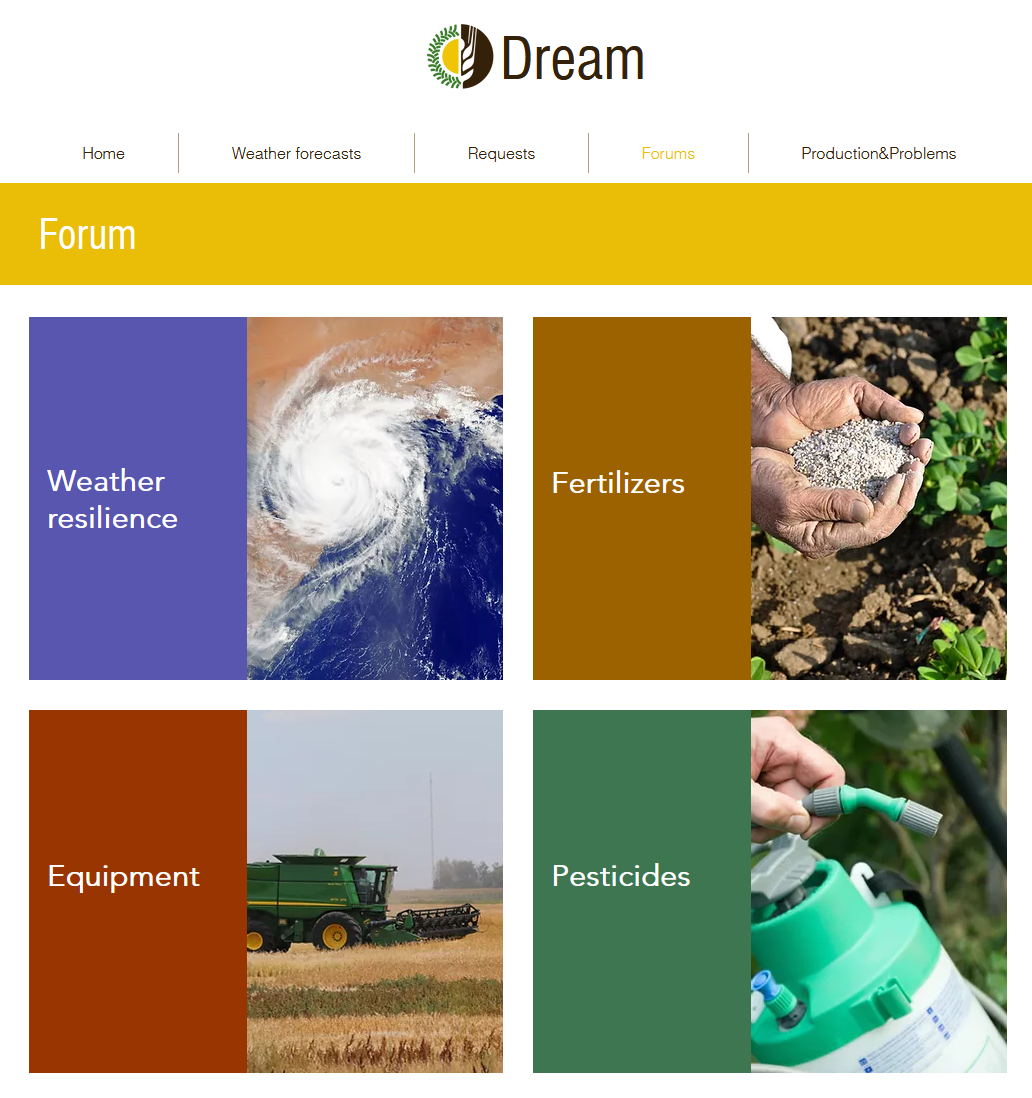
\includegraphics[width=0.7\textwidth]{images/UserInterfaces/Farmer/Forum/ForumHomePageWeb.png}
            \quad
            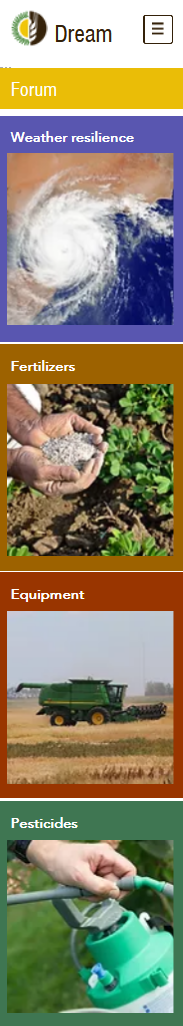
\includegraphics[width=0.2\textwidth]{images/UserInterfaces/Farmer/Forum/ForumHomePageApp.png}
            \quad
            \caption{\label{fig:farmerForumHomePage}Farmer Forum Home Page; web on the left, app on the right}
        \end{figure}
        \newpage
        \begin{figure} [h]
            \centering
            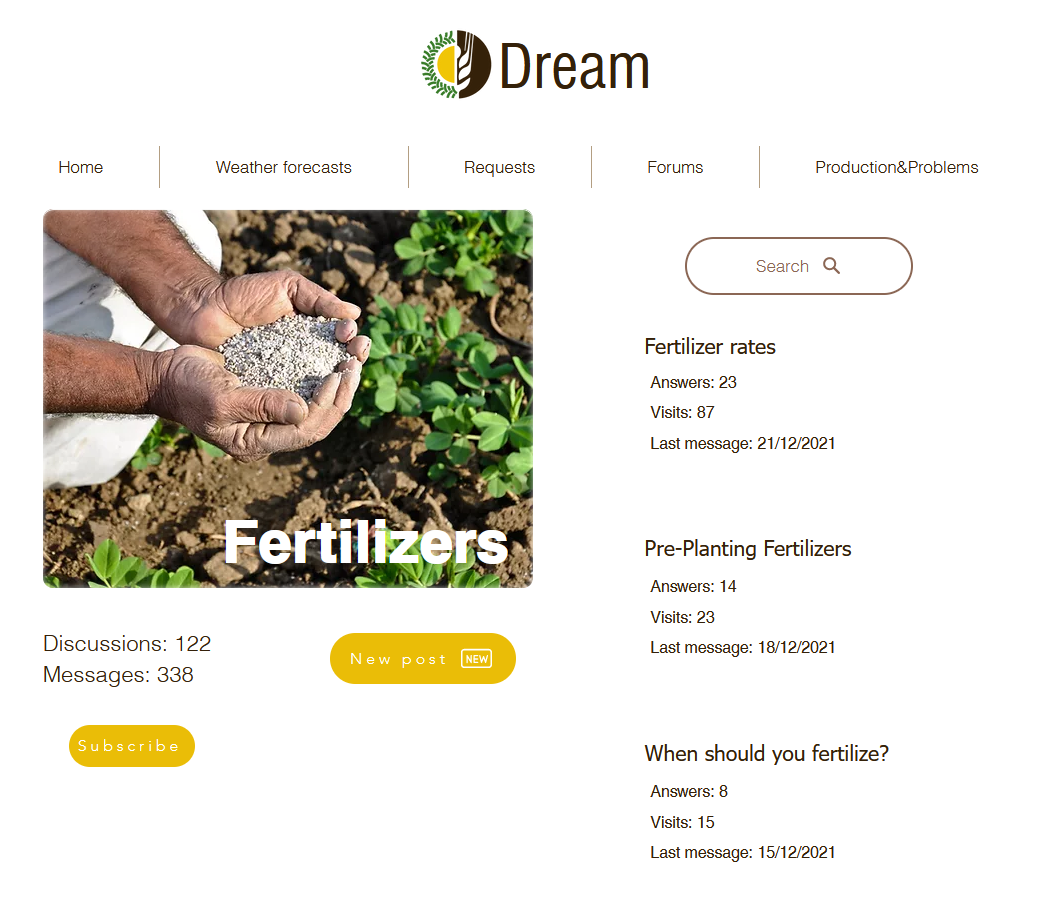
\includegraphics[width=0.7\textwidth]{images/UserInterfaces/Farmer/Forum/ForumPageSubWeb.png}
            \quad
            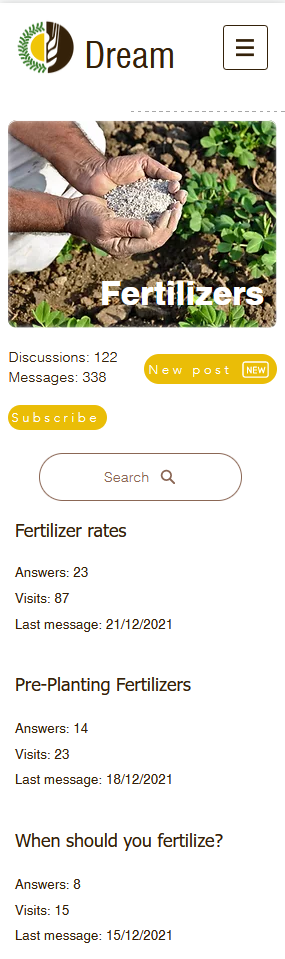
\includegraphics[width=0.2\textwidth]{images/UserInterfaces/Farmer/Forum/ForumPageSubApp.png}
            \quad
            \caption{\label{fig:farmerForumPageSub}Farmer Forum Page Subscribe; web on the left, app on the right}
        \end{figure}
        \newpage
        \begin{figure} [h]
            \centering
            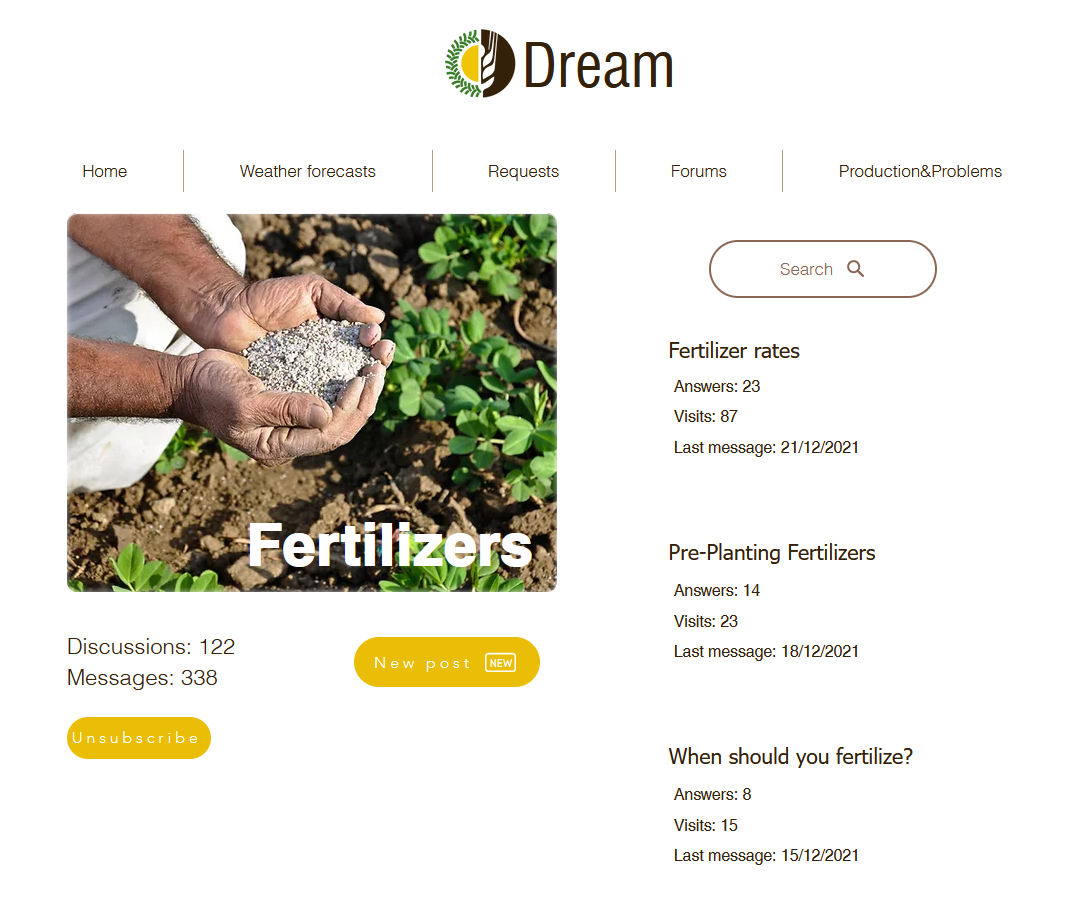
\includegraphics[width=0.7\textwidth]{images/UserInterfaces/Farmer/Forum/ForumPageUnsubWeb.png}
            \quad
            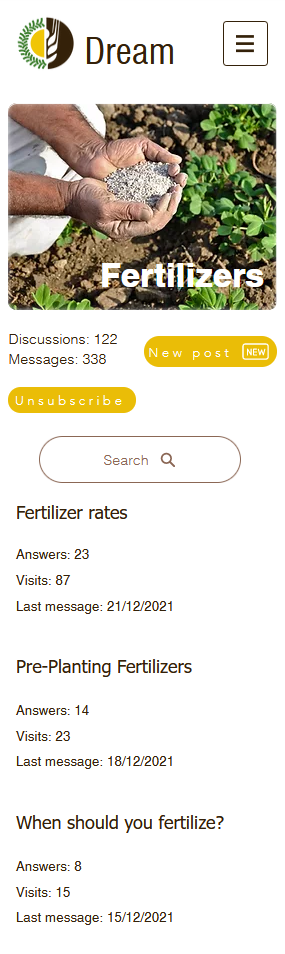
\includegraphics[width=0.2\textwidth]{images/UserInterfaces/Farmer/Forum/ForumPageUnsubApp.png}
            \quad
            \caption{\label{fig:farmerForumPageUnsub}Farmer Forum Page Unsubscribe; web on the left, app on the right}
        \end{figure}
        \newpage
        \begin{figure} [h]
            \centering
            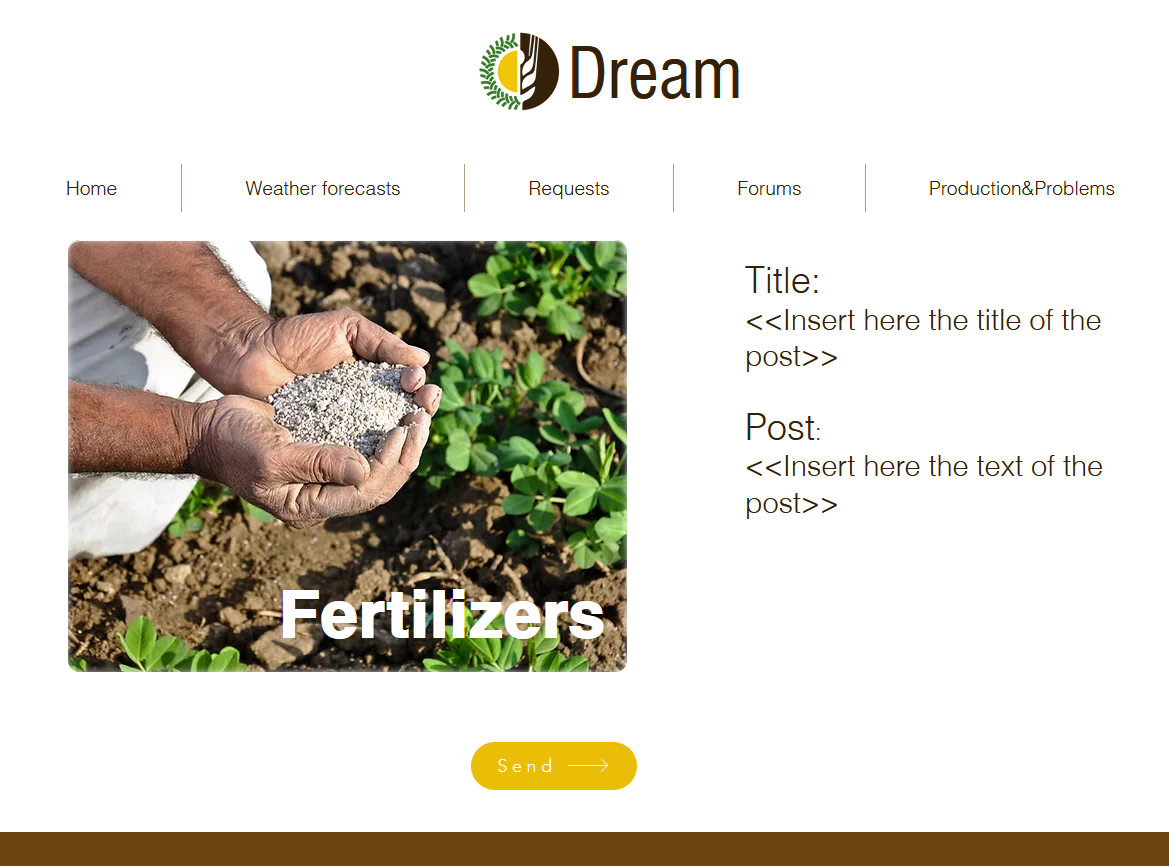
\includegraphics[width=0.6\textwidth]{images/UserInterfaces/Farmer/Forum/NewPostWeb.png}
            \quad
            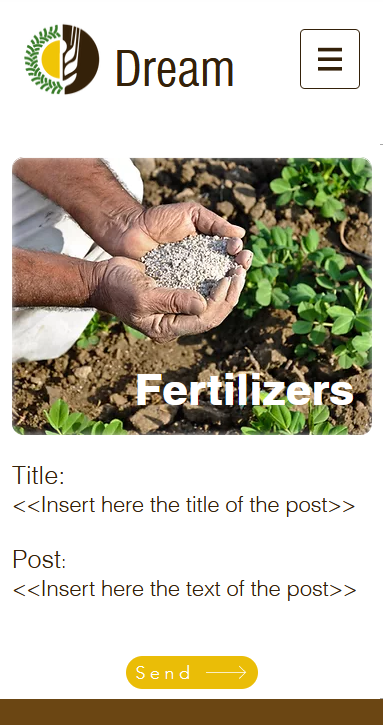
\includegraphics[width=0.2\textwidth]{images/UserInterfaces/Farmer/Forum/NewPostApp.png}
            \quad
            \caption{\label{fig:farmerForumNewPost}Farmer Forum New Post; web on the left, app on the right}
        \end{figure}
        \newpage
        \begin{figure} [h]
            \centering
            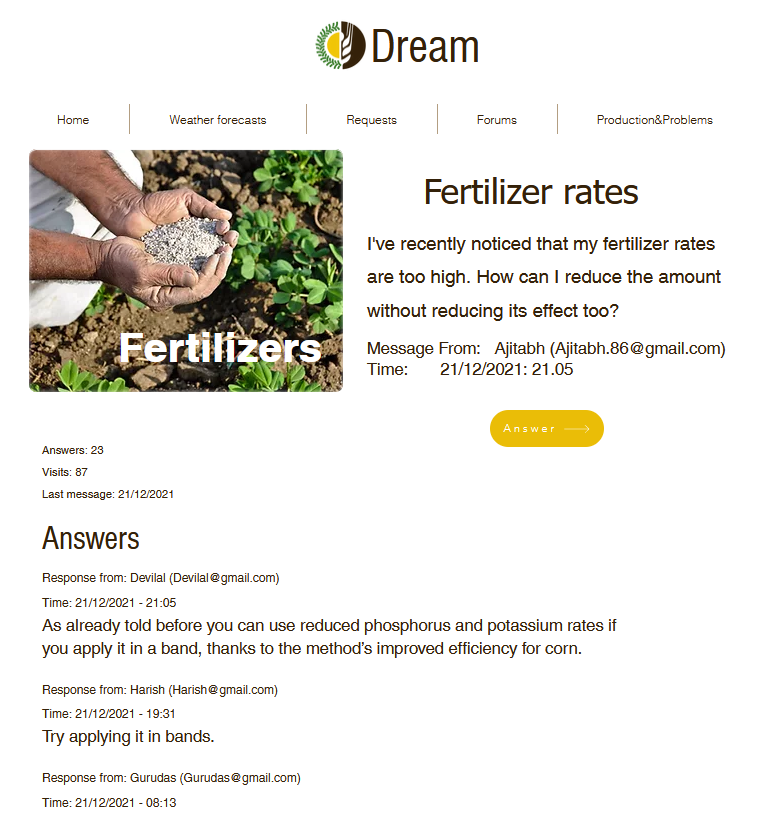
\includegraphics[width=0.7\textwidth]{images/UserInterfaces/Farmer/Forum/SpecificPostWeb.png}
            \quad
            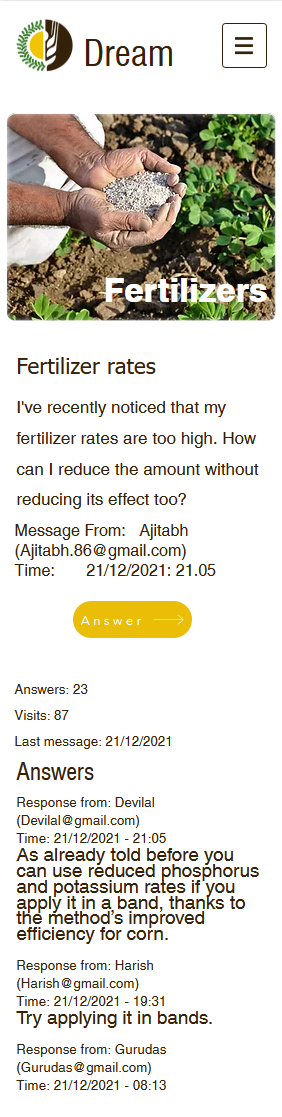
\includegraphics[width=0.2\textwidth]{images/UserInterfaces/Farmer/Forum/SpecificPostApp.png}
            \quad
            \caption{\label{fig:farmerForumSpecificPost}Farmer Forum Specific Post; web on the left, app on the right}
        \end{figure}
        \newpage
        \begin{figure} [h]
            \centering
            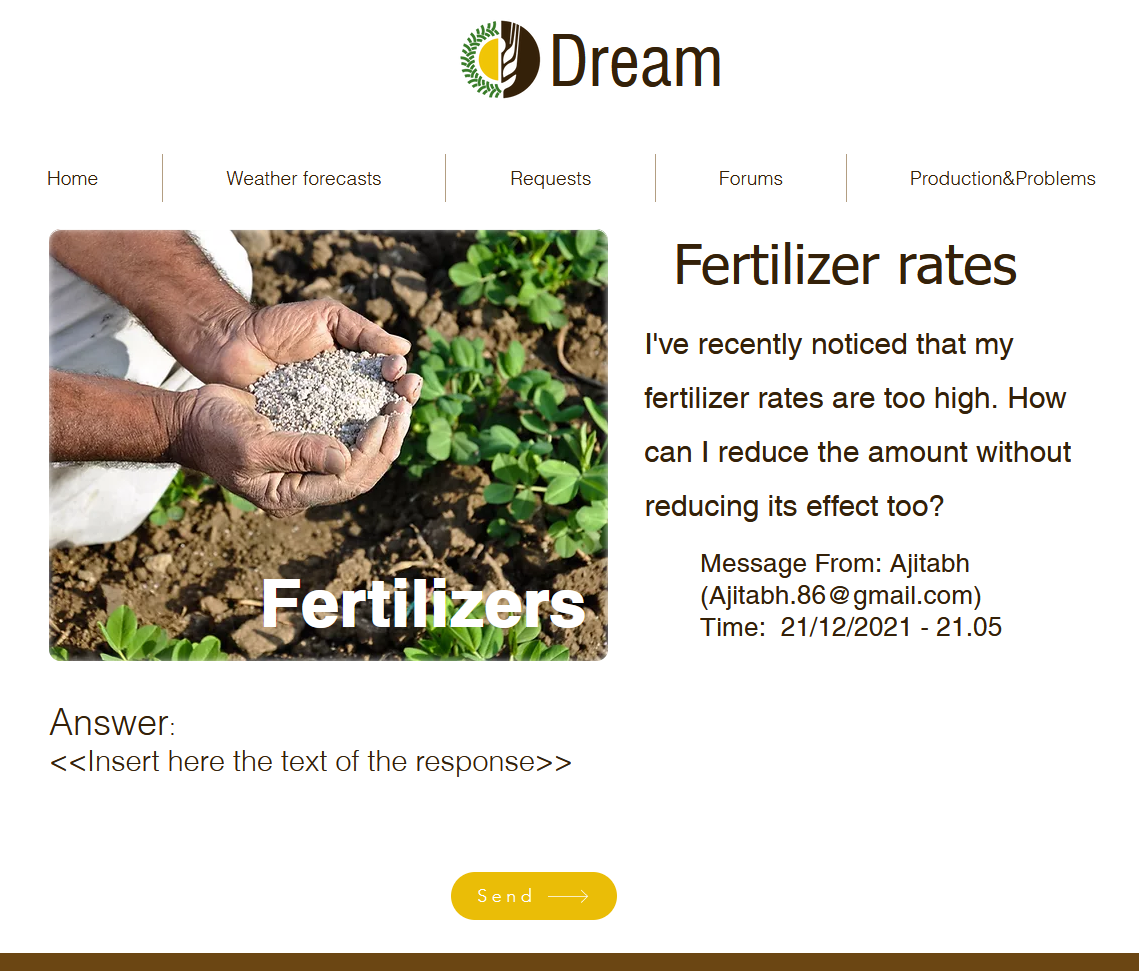
\includegraphics[width=0.7\textwidth]{images/UserInterfaces/Farmer/Forum/ResponseInAPostWeb.png}
            \quad
            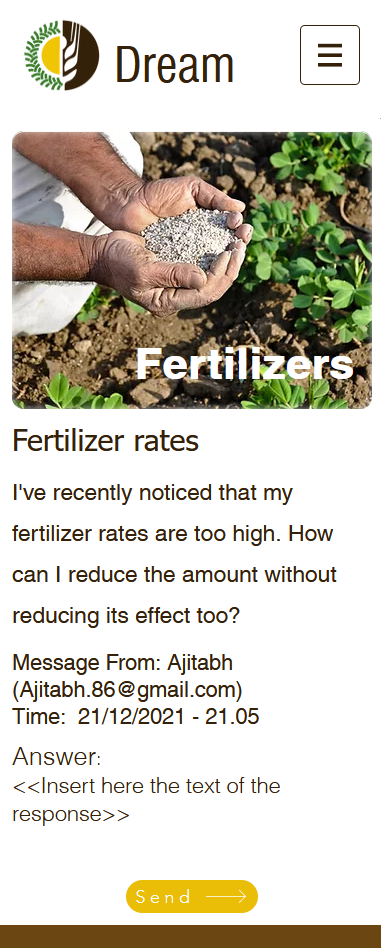
\includegraphics[width=0.2\textwidth]{images/UserInterfaces/Farmer/Forum/ResponseInAPostApp.png}
            \quad
            \caption{\label{fig:farmerForumPostResponse}Farmer Forum Response in a Post; web on the left, app on the right}
        \end{figure}
    
    
    \newpage
    
    
    \begin{itemize}
        \item \textbf{Farmer Help and Suggestions}
    \end{itemize}
        \begin{figure} [h]
            \centering
            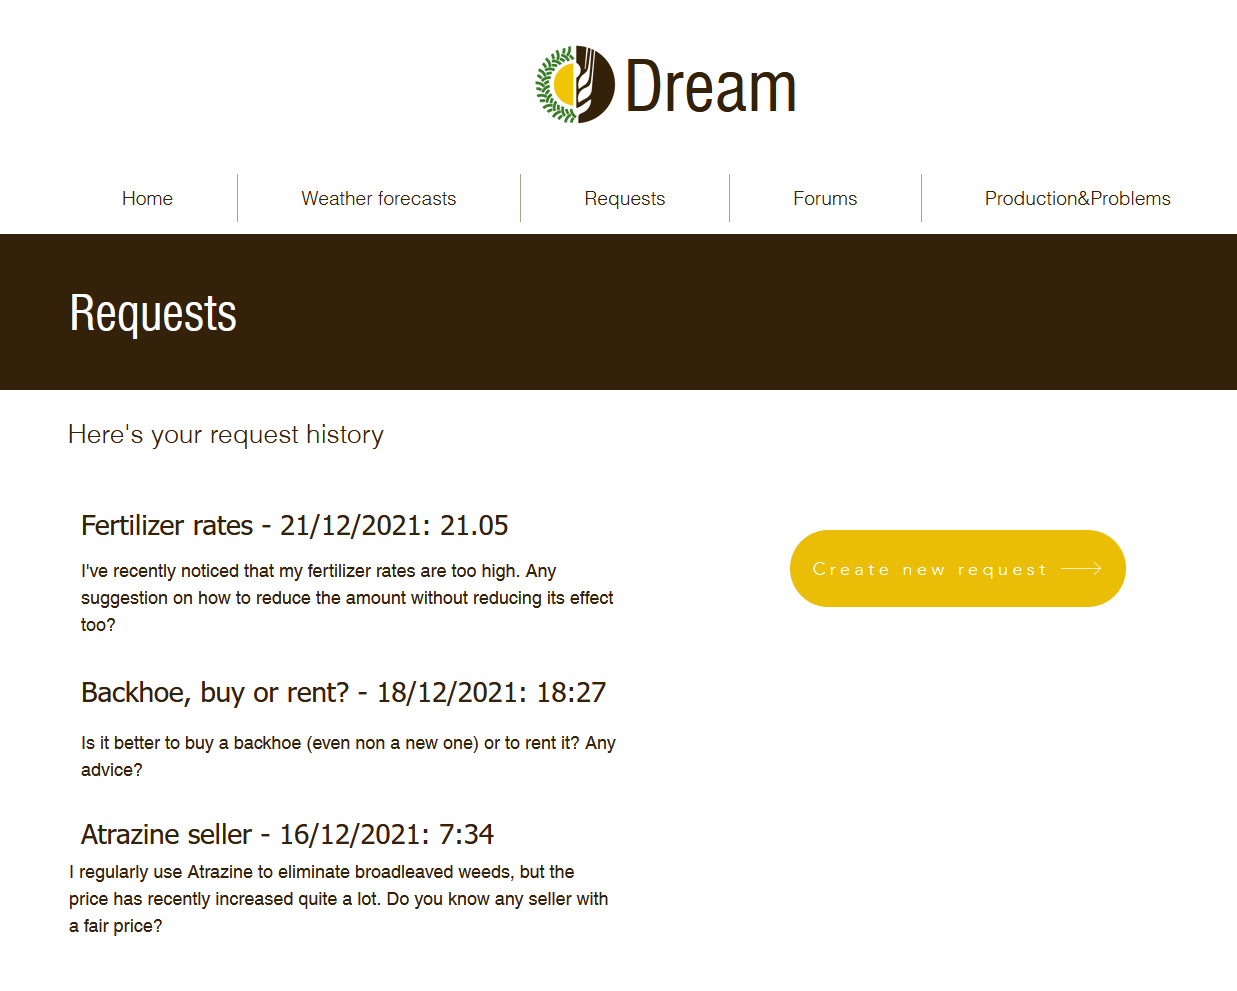
\includegraphics[width=0.7\textwidth]{images/UserInterfaces/Farmer/HelpAndSuggestions/RequestHistoryWeb.png}
            \quad
            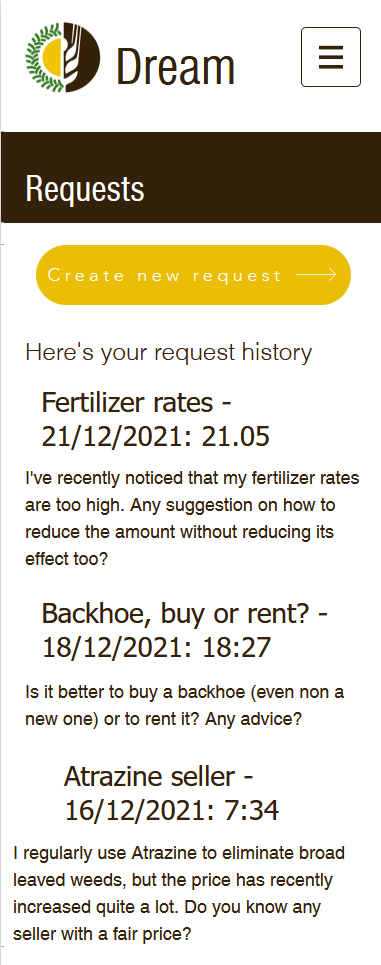
\includegraphics[width=0.2\textwidth]{images/UserInterfaces/Farmer/HelpAndSuggestions/RequestHistoryApp.png}
            \quad
            \caption{\label{fig:farmerHelpHistory}Farmer Help and Suggestions Request History; web on the left, app on the right}
        \end{figure}
        \newpage
        \begin{figure} [h]
            \centering
            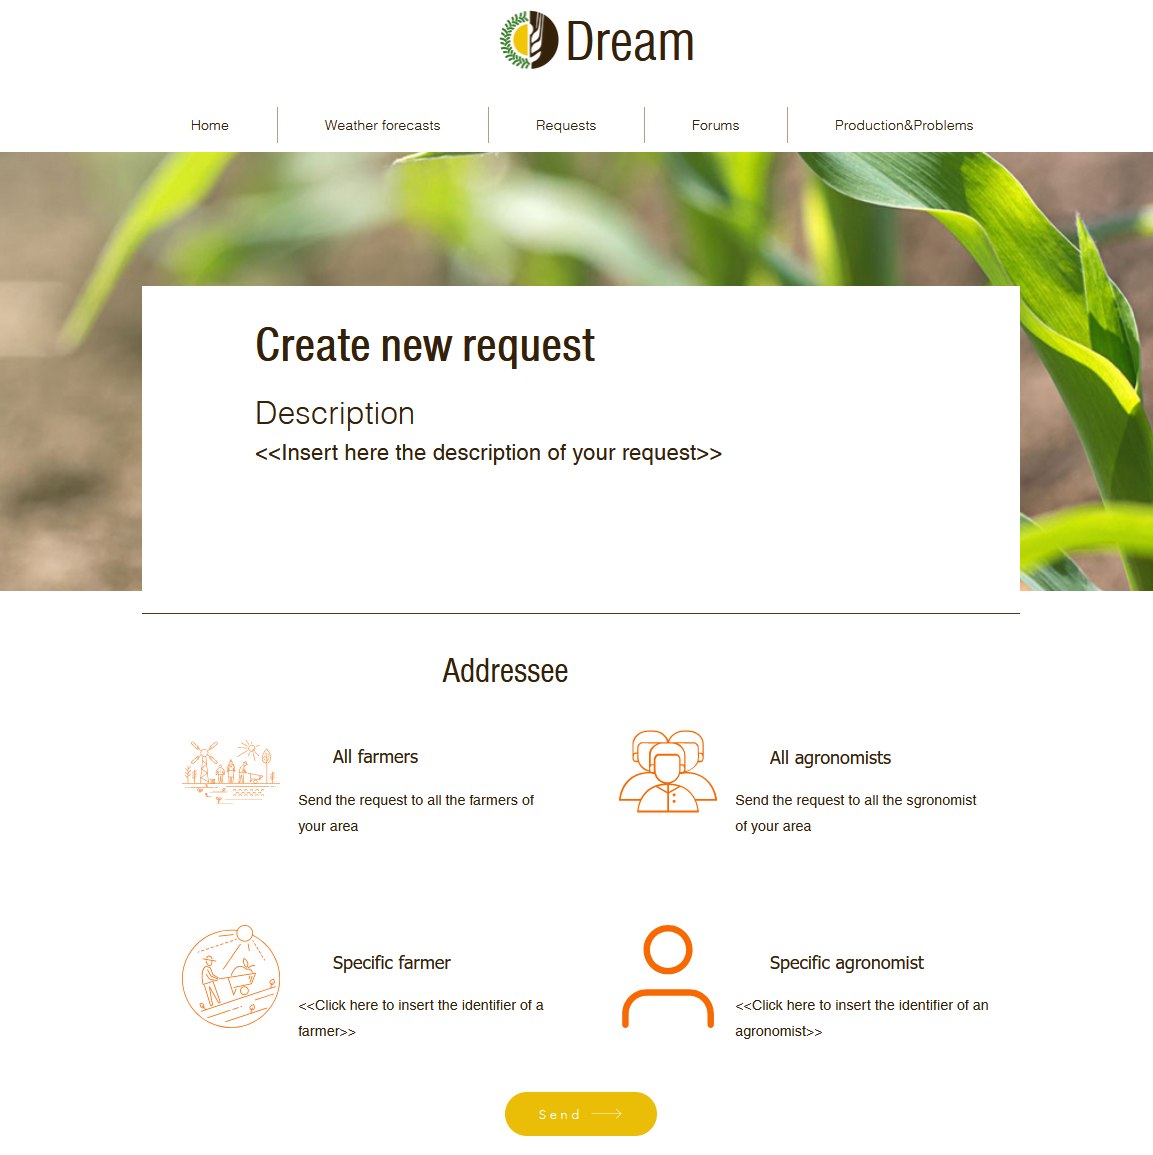
\includegraphics[width=0.7\textwidth]{images/UserInterfaces/Farmer/HelpAndSuggestions/CreateNewRequestWeb.png}
            \quad
            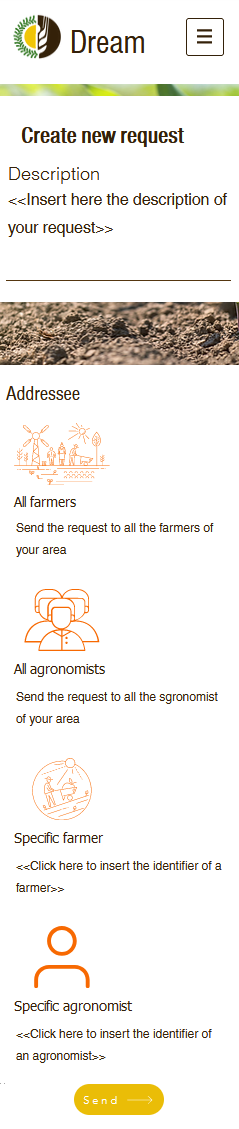
\includegraphics[width=0.2\textwidth]{images/UserInterfaces/Farmer/HelpAndSuggestions/CreateNewRequestApp.png}
            \quad
            \caption{\label{fig:farmerHelpNewRequest}Farmer Help and Suggestions Create New Request; web on the left, app on the right}
        \end{figure}
        \newpage
        \begin{figure} [h]
            \centering
            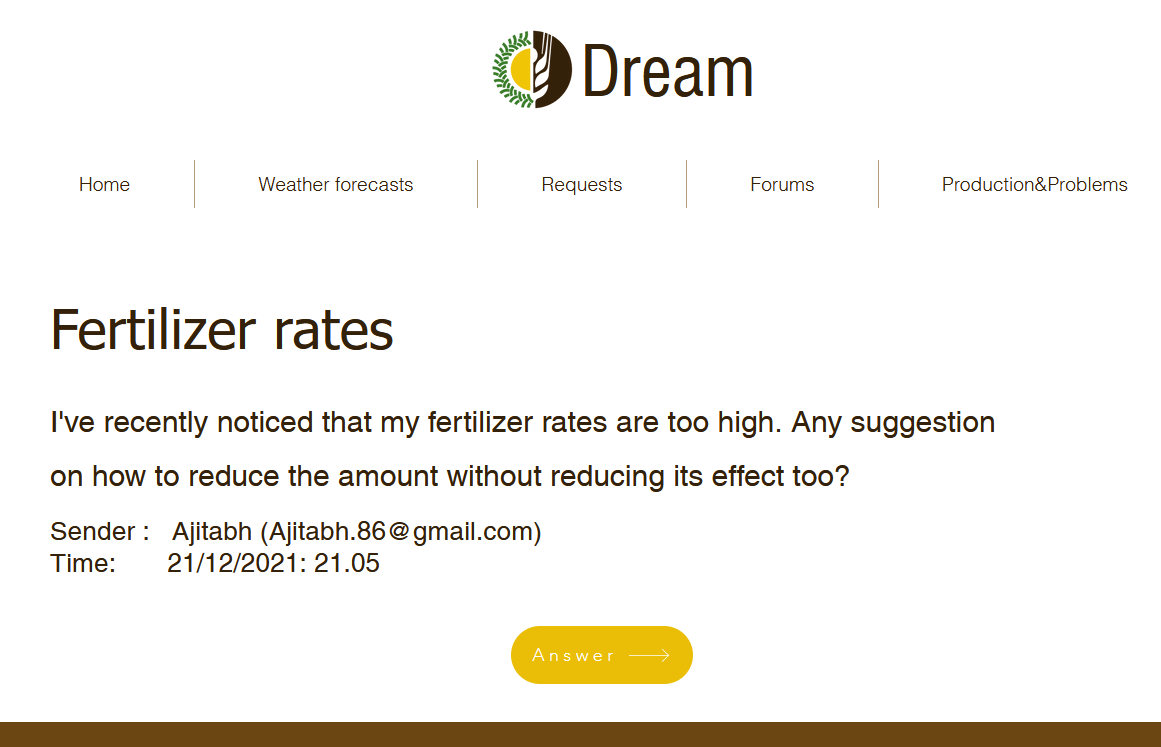
\includegraphics[width=0.7\textwidth]{images/UserInterfaces/Farmer/HelpAndSuggestions/SpecificRequestWeb.png}
            \quad
            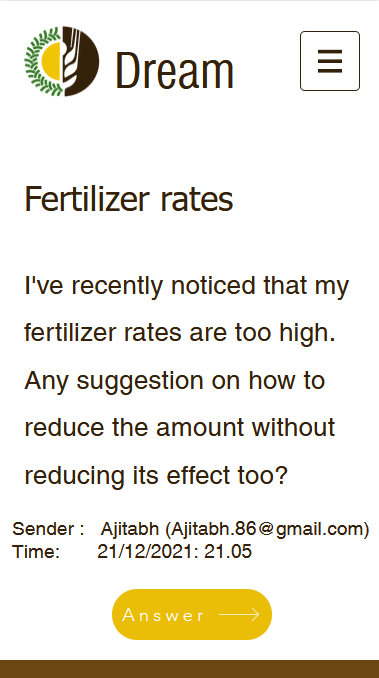
\includegraphics[width=0.2\textwidth]{images/UserInterfaces/Farmer/HelpAndSuggestions/SpecificRequestApp.png}
            \quad
            \caption{\label{fig:farmerHelpSpecificRequest}Farmer Help and Suggestions Specific Request; web on the left, app on the right}
        \end{figure}
        \newpage
        \begin{figure} [h]
            \centering
            \includegraphics[width=0.7\textwidth]{images/UserInterfaces/Farmer/HelpAndSuggestions/ResponseSpecificRequestWeb.png}
            \quad
            \includegraphics[width=0.2\textwidth]{images/UserInterfaces/Farmer/HelpAndSuggestions/ResponseSpecificRequestApp.png}
            \quad
            \caption{\label{fig:farmerHelpResponseSpecificRequest}Farmer Help and Suggestions Response to a Specific Request; web on the left, app on the right}
        \end{figure}
    
    \newpage
    
    \begin{itemize}
        \item \textbf{Farmer Personalized Suggestions}
    \end{itemize}
        \begin{figure} [h]
            \centering
            \includegraphics[width=0.7\textwidth]{images/UserInterfaces/Farmer/PersonalizedSuggestions/PersonalizedSuggestionsWeb.png}
            \quad
            \includegraphics[width=0.2\textwidth]{images/UserInterfaces/Farmer/PersonalizedSuggestions/PersonalizedSuggestionsApp.png}
            \quad
            \caption{\label{fig:farmerPersonalizedSuggestions}Farmer Personalized Suggestions; web on the left, app on the right}
        \end{figure}
        \newpage
        \begin{figure} [h]
            \centering
            \includegraphics[width=0.7\textwidth]{images/UserInterfaces/Farmer/PersonalizedSuggestions/SpecificSuggestionWeb.png}
            \quad
            \includegraphics[width=0.2\textwidth]{images/UserInterfaces/Farmer/PersonalizedSuggestions/SpecificSuggestionApp.png}
            \quad
            \caption{\label{fig:farmerPersonalizedSuggestionsSpecific}Farmer Specific Personalized Suggestions; web on the left, app on the right}
        \end{figure}
        \newpage
        
    \newpage
    
    \begin{itemize}
        \item \textbf{Farmer Production and Problems}
    \end{itemize}
        \begin{figure} [h]
            \centering
            \includegraphics[width=0.7\textwidth]{images/UserInterfaces/Farmer/ProductionAndProblems/ProductionProblemsWeb.png}
            \quad
            \includegraphics[width=0.2\textwidth]{images/UserInterfaces/Farmer/ProductionAndProblems/ProductionProblemsApp.png}
            \quad
            \caption{\label{fig:farmerProduction}Farmer Production and Problems; web on the left, app on the right}
        \end{figure}
        \newpage
        \begin{figure} [h]
            \centering
            \includegraphics[width=0.7\textwidth]{images/UserInterfaces/Farmer/ProductionAndProblems/ProductionHistoryWeb.png}
            \quad
            \includegraphics[width=0.2\textwidth]{images/UserInterfaces/Farmer/ProductionAndProblems/ProductionHistoryApp.png}
            \quad
            \caption{\label{fig:farmerProductionHistory}Farmer Production History; web on the left, app on the right}
        \end{figure}
        \newpage
        \begin{figure} [h]
            \centering
            \includegraphics[width=0.7\textwidth]{images/UserInterfaces/Farmer/ProductionAndProblems/InsertsProductionDataWeb.png}
            \quad
            \includegraphics[width=0.2\textwidth]{images/UserInterfaces/Farmer/ProductionAndProblems/InsertProductionDataApp.png}
            \quad
            \caption{\label{fig:farmerInsertProduction}Farmer Insert Production Data; web on the left, app on the right}
        \end{figure}
        \newpage
        \begin{figure} [h]
            \centering
            \includegraphics[width=0.7\textwidth]{images/UserInterfaces/Farmer/ProductionAndProblems/ReportProblemWeb.png}
            \quad
            \includegraphics[width=0.2\textwidth]{images/UserInterfaces/Farmer/ProductionAndProblems/ReportProblemApp.png}
            \quad
            \caption{\label{fig:farmerReportProblem}Farmer Report a Problem; web on the left, app on the right}
        \end{figure}
    
    
    \newpage
    

    \begin{itemize}
        \item \textbf{Farmer Weather}
    \end{itemize}
        \begin{figure} [h]
            \centering
            \includegraphics[width=0.7\textwidth]{images/UserInterfaces/Farmer/Weather/DaysForecastWeb.png}
            \quad
            \includegraphics[width=0.2\textwidth]{images/UserInterfaces/Farmer/Weather/DaysForecastApp.png}
            \quad
            \caption{\label{fig:farmerWeatherDay}Farmer Days Forecasts; web on the left, app on the right}
        \end{figure}
        \newpage
        \begin{figure} [h]
            \centering
            \includegraphics[width=0.7\textwidth]{images/UserInterfaces/Farmer/Weather/HoursForecastWeb.png}
            \quad
            \includegraphics[width=0.2\textwidth]{images/UserInterfaces/Farmer/Weather/HoursForecastApp.png}
            \quad
            \caption{\label{fig:farmerWeatherHaour}Farmer Hours Forecasts; web on the left, app on the right}
        \end{figure}
    
    
    \newpage
    
    
    \subsection{Agronomist}
    
    \begin{itemize}
        \item \textbf{Agronomist Sign In}
    \end{itemize}
        \begin{figure} [h]
            \centering
            \includegraphics[width=0.7\textwidth]{images/UserInterfaces/Agronomist/AgronomistSignInWeb.png}
            \quad
            \includegraphics[width=0.2\textwidth]{images/UserInterfaces/Agronomist/AgronomistSignInApp.png}
            \quad
            \caption{\label{fig:agronomistSignIn}Agronomist Sign In; web on the left, app on the right}
        \end{figure}
    
    \newpage

    \begin{itemize}
        \item \textbf{Agronomist Home Page}
    \end{itemize}
        \begin{figure} [h]
            \centering
            \includegraphics[width=0.7\textwidth]{images/UserInterfaces/Agronomist/AgronomistHomePageWeb.png}
            \quad
            \includegraphics[width=0.2\textwidth]{images/UserInterfaces/Agronomist/AgronomistHomePageApp.png}
            \quad
            \caption{\label{fig:agronomistHomePage}Agronomist Home Page; web on the left, app on the right}
        \end{figure}
    
    
    \newpage
    
    
    \begin{itemize}
        \item \textbf{Agronomist Daily Plan}
    \end{itemize}
        \begin{figure} [h]
            \centering
            \includegraphics[width=0.7\textwidth]{images/UserInterfaces/Agronomist/DailyPlan/DailyPlanHomePageWeb.png}
            \quad
            \includegraphics[width=0.2\textwidth]{images/UserInterfaces/Agronomist/DailyPlan/DailyPlanHomePageApp.png}
            \quad
            \caption{\label{fig:agronomistDPHomePage}Agronomist Daily Plan Home Page; web on the left, app on the right}
        \end{figure}
        \newpage
        \begin{figure} [h]
            \centering
            \includegraphics[width=0.7\textwidth]{images/UserInterfaces/Agronomist/DailyPlan/ConfirmDeviationsWeb.png}
            \quad
            \includegraphics[width=0.2\textwidth]{images/UserInterfaces/Agronomist/DailyPlan/ConfirmDeviationsApp.png}
            \quad
            \caption{\label{fig:agronomistDPConfirmDeviations}Agronomist Confirm Daily Plan or Specify Deviations; web on the left, app on the right}
        \end{figure}
        \newpage
        \begin{figure} [h]
            \centering
            \includegraphics[width=0.7\textwidth]{images/UserInterfaces/Agronomist/DailyPlan/SpecificDayConfirmDeviationsWeb.png}
            \quad
            \includegraphics[width=0.2\textwidth]{images/UserInterfaces/Agronomist/DailyPlan/SpecificDayConfirmDeviationsApp.png}
            \quad
            \caption{\label{fig:agronomistDPConfirmDeviationsSpecific}Agronomist Specific Day Confirm Daily Plan or Specify Deviations; web on the left, app on the right}
        \end{figure}
        \newpage
        \begin{figure} [h]
            \centering
            \includegraphics[width=0.7\textwidth]{images/UserInterfaces/Agronomist/DailyPlan/ConfirmedExecutionWeb.png}
            \quad
            \includegraphics[width=0.2\textwidth]{images/UserInterfaces/Agronomist/DailyPlan/ConfirmedExecutionApp.png}
            \quad
            \caption{\label{fig:agronomistDPConfirmedExecution}Agronomist Confirmed Execution of Daily Plan; web on the left, app on the right}
        \end{figure}
        \newpage
        \begin{figure} [h]
            \centering
            \includegraphics[width=0.7\textwidth]{images/UserInterfaces/Agronomist/DailyPlan/InsertWeb.png}
            \quad
            \includegraphics[width=0.2\textwidth]{images/UserInterfaces/Agronomist/DailyPlan/InsertApp.png}
            \quad
            \caption{\label{fig:agronomistDPInsert}Agronomist Insert Daily Plan; web on the left, app on the right}
        \end{figure}
        \newpage
        \begin{figure} [h]
            \centering
            \includegraphics[width=0.7\textwidth]{images/UserInterfaces/Agronomist/DailyPlan/UpdateWeb.png}
            \quad
            \includegraphics[width=0.2\textwidth]{images/UserInterfaces/Agronomist/DailyPlan/UpdateApp.png}
            \quad
            \caption{\label{fig:agronomistDPUpdate}Agronomist Update Daily Plan; web on the left, app on the right}
        \end{figure}
        \newpage
        \begin{figure} [h]
            \centering
            \includegraphics[width=0.7\textwidth]{images/UserInterfaces/Agronomist/DailyPlan/UpdateButtonWeb.png}
            \quad
            \includegraphics[width=0.2\textwidth]{images/UserInterfaces/Agronomist/DailyPlan/UpdateButtonApp.png}
            \quad
            \caption{\label{fig:agronomistDPUpdateButton}Agronomist Update Button; web on the left, app on the right}
        \end{figure}
    
    
    \newpage
    
    
    \begin{itemize}
        \item \textbf{Agronomist Visualize Farmers' performance}
    \end{itemize}
        \begin{figure} [h]
            \centering
            \includegraphics[width=0.7\textwidth]{images/UserInterfaces/Agronomist/FarmersPerformance/FarmersPerformanceWeb.png}
            \quad
            \includegraphics[width=0.2\textwidth]{images/UserInterfaces/Agronomist/FarmersPerformance/FarmersPerformanceApp.png}
            \quad
            \caption{\label{fig:agronomistFarmersPerformance}Agronomist Visualize Farmers' Performance; web on the left, app on the right}
        \end{figure}
        \newpage
        \begin{figure} [h]
            \centering
            \includegraphics[width=0.7\textwidth]{images/UserInterfaces/Agronomist/FarmersPerformance/SpecificPerformanceWeb.png}
            \quad
            \includegraphics[width=0.2\textwidth]{images/UserInterfaces/Agronomist/FarmersPerformance/SpecificPerformanceApp.png}
            \quad
            \caption{\label{fig:agronomistSpecificFarmersPerformance}Agronomist Visualize Specific Farmers' Performance; web on the left, app on the right}
        \end{figure}
    
    
    \newpage
    
    
    \begin{itemize}
        \item \textbf{Agronomist Visualize Farmers' performance}
    \end{itemize}
        \begin{figure} [h]
            \centering
            \includegraphics[width=0.7\textwidth]{images/UserInterfaces/Agronomist/Requests/RequestsWeb.png}
            \quad
            \includegraphics[width=0.2\textwidth]{images/UserInterfaces/Agronomist/Requests/RequestsApp.png}
            \quad
            \caption{\label{fig:agronomistRequests}Agronomist Requests Home Page; web on the left, app on the right}
        \end{figure}
        \newpage
        \begin{figure} [h]
            \centering
            \includegraphics[width=0.7\textwidth]{images/UserInterfaces/Agronomist/Requests/SpecificRequestWeb.png}
            \quad
            \includegraphics[width=0.2\textwidth]{images/UserInterfaces/Agronomist/Requests/SpecificRequestApp.png}
            \quad
            \caption{\label{fig:agronomistRequest}Agronomist Specific Request; web on the left, app on the right}
        \end{figure}
        \newpage
        \begin{figure} [h]
            \centering
            \includegraphics[width=0.7\textwidth]{images/UserInterfaces/Agronomist/Requests/RespondWeb.png}
            \quad
            \includegraphics[width=0.2\textwidth]{images/UserInterfaces/Agronomist/Requests/RespondApp.png}
            \quad
            \caption{\label{fig:agronomistRespond}Agronomist Respond to a Request; web on the left, app on the right}
        \end{figure}
        \newpage
        
    
    \subsection{Policy Maker}
    
    \begin{itemize}
        \item \textbf{Policy Maker Sign In}
    \end{itemize}
        \begin{figure} [h]
            \centering
            \includegraphics[width=0.7\textwidth]{images/UserInterfaces/PolicyMaker/PolicyMakerSignInWeb.png}
            \quad
            \includegraphics[width=0.2\textwidth]{images/UserInterfaces/PolicyMaker/PolicyMakerSignInApp.png}
            \quad
            \caption{\label{fig:policyMakerSignIn}Policy Maker Sign In; web on the left, app on the right}
        \end{figure}
    
    \newpage

    \begin{itemize}
        \item \textbf{Policy Maker Home Page}
    \end{itemize}
        \begin{figure} [h]
            \centering
            \includegraphics[width=0.7\textwidth]{images/UserInterfaces/PolicyMaker/PolicyMakerHomePageWeb.png}
            \quad
            \includegraphics[width=0.2\textwidth]{images/UserInterfaces/PolicyMaker/PolicyMakerHomePageApp.png}
            \quad
            \caption{\label{fig:policyMakerHomePage}Policy Maker Home Page; web on the left, app on the right}
        \end{figure}
    
    
    \newpage
    
    
    \begin{itemize}
        \item \textbf{Policy Maker Visualize Farmers' performance}
    \end{itemize}
        \begin{figure} [h]
            \centering
            \includegraphics[width=0.7\textwidth]{images/UserInterfaces/PolicyMaker/FarmersPerformance/FarmersPerformanceWeb.png}
            \quad
            \includegraphics[width=0.2\textwidth]{images/UserInterfaces/PolicyMaker/FarmersPerformance/FarmersPerformanceApp.png}
            \quad
            \caption{\label{fig:policyMakerVisualizeFarmers}Policy Maker Visualize Farmers' Performance; web on the left, app on the right}
        \end{figure}
        \newpage
        \begin{figure} [h]
            \centering
            \includegraphics[width=0.7\textwidth]{images/UserInterfaces/PolicyMaker/FarmersPerformance/AskButtonWeb.png}
            \quad
            \includegraphics[width=0.2\textwidth]{images/UserInterfaces/PolicyMaker/FarmersPerformance/AskButtonApp.png}
            \quad
            \caption{\label{fig:policyMakerAskBestPracticesFarmersPerformance}Policy Maker Ask for Best Practice; web on the left, app on the right}
        \end{figure}
    
    \newpage
    
    \begin{itemize}
        \item \textbf{Policy Maker Best Practices}
    \end{itemize}
        \begin{figure} [h]
            \centering
            \includegraphics[width=0.7\textwidth]{images/UserInterfaces/PolicyMaker/BestPractices/BestPracticesWeb.png}
            \quad
            \includegraphics[width=0.2\textwidth]{images/UserInterfaces/PolicyMaker/BestPractices/BestPracticesApp.png}
            \quad
            \caption{\label{fig:policyMakerBestPractices}Policy Maker Best Practices Home Page; web on the left, app on the right}
        \end{figure}
        \newpage
        \begin{figure} [h]
            \centering
            \includegraphics[width=0.7\textwidth]{images/UserInterfaces/PolicyMaker/BestPractices/RequestBestPracticesWeb.png}
            \quad
            \includegraphics[width=0.2\textwidth]{images/UserInterfaces/PolicyMaker/BestPractices/RequestBestPracticesApp.png}
            \quad
            \caption{\label{fig:policyMakerAskBestPractices}Policy Maker Ask for Best Practices through Best Practices; web on the left, app on the right}
        \end{figure}
    
    
    \newpage
    \newpage
    
        
\newpage


    \subsection{Flow of functionalities}
    
        \subsubsection{User Sign Up and Login}
            \begin{figure} [h]
                \centering
                \includegraphics[width=1\textwidth]{images/UserInterfaces/MapsFunctionalities/1. UserSignUpAndLogin.jpg}
                \caption{\label{fig:UserSignUpLogin}User Sign Up and Login}
            \end{figure}
    
        \newpage
        
        
        \subsubsection{Farmer visualizes weather forecasts}
            \begin{figure} [h]
                \centering
                \includegraphics[width=1\textwidth]{images/UserInterfaces/MapsFunctionalities/2. FarmerVisualizeWeatherForecasts.jpg}
                \caption{\label{fig:FarmerWeatherForecasts}Farmer visualizes weather forecasts}
            \end{figure}
            
        
        
        \subsubsection{Farmer visualizes personalized suggestions}
            \begin{figure} [h]
                \centering
                \includegraphics[width=1\textwidth]{images/UserInterfaces/MapsFunctionalities/3. FarmerVisualizePersonalizedSuggestions.jpg}
                \caption{\label{fig:FarmerPersonalizedSuggestions}Farmer visualizes personalized suggestions}
            \end{figure}
    
        \newpage

        
        \subsubsection{Farmer inserts production data}
            \begin{figure} [h]
                \centering
                \includegraphics[width=1\textwidth]{images/UserInterfaces/MapsFunctionalities/4. FarmerInsertProductionData.jpg}
                \caption{\label{fig:FarmerProductionData}Farmer inserts production data}
            \end{figure}
    
        
        \subsubsection{Farmer reports a problem}
            \begin{figure} [h]
                \centering
                \includegraphics[width=1\textwidth]{images/UserInterfaces/MapsFunctionalities/5. FarmerReportAProblem.jpg}
                \caption{\label{fig:FarmerReportsProblem}Farmer reports a problem}
            \end{figure}
    
        \newpage
        
        
        \subsubsection{Farmer requests for help and suggestions}
            \begin{figure} [h]
                \centering
                \includegraphics[width=1\textwidth]{images/UserInterfaces/MapsFunctionalities/6. FarmerRequestsHelpAndSuggestions.jpg}
                \caption{\label{fig:FarmerRequestsHelp}Farmer requests for help and suggestions}
            \end{figure}
    
        
        
        \subsubsection{Farmer responds to a request for help and suggestions}
            \begin{figure} [h]
                \centering
                \includegraphics[width=1\textwidth]{images/UserInterfaces/MapsFunctionalities/7. FarmerRespondsHelpAndSuggestions.jpg}
                \caption{\label{fig:FarmerResponseHelp}Farmer responds to a request for help and suggestions}
            \end{figure}
    
        \newpage
        
        
        \subsubsection{Farmer writes a new post on forum}
            \begin{figure} [h]
                \centering
                \includegraphics[width=1\textwidth]{images/UserInterfaces/MapsFunctionalities/8. FarmerWritesPostOnForum.jpg}
                \caption{\label{fig:FarmerWritesPost}Farmer writes a new post on forum}
            \end{figure}
        
        
        \subsubsection{Farmer responds on a discussion forum}
            \begin{figure} [h]
                \centering
                \includegraphics[width=1\textwidth]{images/UserInterfaces/MapsFunctionalities/9. FarmerRespondsOnForum.jpg}
                \caption{\label{fig:FarmerRespondsForum}Farmer responds on a discussion forum}
            \end{figure}
            
            
        \subsubsection{Farmer inserts best practices}
            \begin{figure} [h]
                \centering
                \includegraphics[width=1\textwidth]{images/UserInterfaces/MapsFunctionalities/12. FarmerInsertsBestPractices.jpg}
                \caption{\label{fig:FarmerInsertBestPractice}Farmer inserts best practices}
            \end{figure}
    
        \newpage
        
        \subsubsection{Farmer subscribes to a topic}
            \begin{figure} [h]
                \centering
                \includegraphics[width=1\textwidth]{images/UserInterfaces/MapsFunctionalities/10. FarmerSubscribesTopic.jpg}
                \caption{\label{fig:FarmerSubscribesTopic}Farmer subscribes to a topic}
            \end{figure}
        
        
        \subsubsection{Farmer unsubscribes from a topic}
            \begin{figure} [h]
                \centering
                \includegraphics[width=1\textwidth]{images/UserInterfaces/MapsFunctionalities/11. FarmerUnsubscribesFromTopic.jpg}
                \caption{\label{fig:FarmerUnSubscribesTopic}Farmer unsubscribes from a topic}
            \end{figure}
        
        
        
        
    
        \newpage
        
        
        
        \subsubsection{Agronomist answers to a request for help and suggestions}
            \begin{figure} [h]
                \centering
                \includegraphics[width=1\textwidth]{images/UserInterfaces/MapsFunctionalities/14. AgronomistAnswersToRequestHelpAndSuggestions.jpg}
                \caption{\label{fig:AgronomistAnswerHelp}Agronomist answers to a request for help and suggestions}
            \end{figure}
    
        
        
        \subsubsection{Agronomist visualizes daily plan}
            \begin{figure} [h]
                \centering
                \includegraphics[width=1\textwidth]{images/UserInterfaces/MapsFunctionalities/15. AgronomistVisualizesDailyPlan.jpg}
                \caption{\label{fig:AgronomistVisualizeDailyPlan}Agronomist visualizes daily plan}
            \end{figure}
    
        \newpage
        
        \subsubsection{Agronomist inserts daily plan}
            \begin{figure} [h]
                \centering
                \includegraphics[width=1\textwidth]{images/UserInterfaces/MapsFunctionalities/17. AgronomistInsertsDailyPlan.jpg}
                \caption{\label{fig:AgronomistInsertDailyPlan}Agronomist inserts daily plan}
            \end{figure}
        
    
        
        \subsubsection{Agronomist updates daily plan}
            \begin{figure} [h]
                \centering
                \includegraphics[width=0.9\textwidth]{images/UserInterfaces/MapsFunctionalities/16. AgronomistUpdatesDailyPlan.jpg}
                \caption{\label{fig:AgronomistUpdateDailyPlan}Agronomist updates daily plan}
            \end{figure}
        
        
        
    
        \newpage
        
        
        \subsubsection{Agronomist confirms execution of daily plan, or specify deviations}
            \begin{figure} [h]
                \centering
                \includegraphics[width=1\textwidth]{images/UserInterfaces/MapsFunctionalities/18. AgronomistConfirmsExecutionOfDailyPlanOrSpecifiesDeviations.jpg}
                \caption{\label{fig:AgronomistCloseDailyPlan}Agronomist confirms execution of daily plan, or specify deviations}
            \end{figure}
        
        
        \subsubsection{Agronomist visualizes farmers' performance (production data)}
            \begin{figure} [h]
                \centering
                \includegraphics[width=1\textwidth]{images/UserInterfaces/MapsFunctionalities/19. AgronomistVisualizesFarmersPerformance.jpg}
                \caption{\label{fig:AgronomistVisualizeProdData}Agronomist visualizes farmers' performance}
            \end{figure}
    
        \newpage
        
        
        
        \subsubsection{Policy Maker visualizes farmers' performance (production data)}
            \begin{figure} [h]
                \centering
                \includegraphics[width=1\textwidth]{images/UserInterfaces/MapsFunctionalities/21. PolicyMakerVisualizeFarmersPerformance.jpg}
                \caption{\label{fig:PolicyMakerVisualizeProdData}Policy Maker visualizes farmers' performance}
            \end{figure}
        
        
        
        \subsubsection{Policy Maker asks for best practices to a farmer}
            \begin{figure} [h]
                \centering
                \includegraphics[width=1\textwidth]{images/UserInterfaces/MapsFunctionalities/22. PolicyMakerAsksForBestPractices.jpg}
                \caption{\label{fig:PolicyMakerAskBestPractice}Policy Maker asks for best practices to a farmer}
            \end{figure}
    
        \newpage
        
        
        \subsubsection{Policy Maker reports a bad performing farmer}
            \begin{figure} [h]
                \centering
                \includegraphics[width=1\textwidth]{images/UserInterfaces/MapsFunctionalities/23. PolicyMakerReportsBadPerformingFarmer.jpg}
                \caption{\label{fig:PolicyMakerReportsBadFarmer}Policy Maker reports a bad performing farmer}
            \end{figure}
    
        \newpage
        
        
        
                
\section{Requirements Traceability}

This section describes the traceability between requirements written in the RASD and modules described in the component diagram.

    \setlength{\parskip}{0em}

    \begin{itemize}
    
        \item \textbf{R1}: The system shall allow the registration of new users of three different types: farmer, agronomists and policy makers.
            \begin{itemize}
                \item \textit{ClientManager}: manages all guest user interaction, letting them signup and login.
            \end{itemize}
        
        \item \textbf{R2}: The system shall elaborate a list of suggestions for the registered farmer user.
            \begin{itemize}
                \item \textit{Farmer Personalized Suggestions}
            \end{itemize}
        
        \item \textbf{R3}: The system shall allow the farmer user to send help or suggestions requests to a selected agronomist user or farmer user.
            \begin{itemize}
                \item \textit{HelpAndSuggestion Controller}
            \end{itemize}
        
        \item \textbf{R4}: The system shall send a notification to the farmer user when he receives requests for best practices or new answers or requests in the help requests or forum threads.
            \begin{itemize}
                \item \textit{EmailManager}: manages triggers that automatically send notification email to the chosen user.
            \end{itemize}

        \item \textbf{R5}: The system shall allow a farmer user to read and respond to threads in the farmer forums.
            \begin{itemize}
                \item \textit{Forum Controller}
            \end{itemize}
            
        \item \textbf{R6}: The system shall allow a farmer to insert production data.
            \begin{itemize}
                \item \textit{Performance data Controller}
            \end{itemize}

        \item \textbf{R7}: The system shall allow the farmer user to respond to a request for best practices.
            \begin{itemize}
                \item \textit{Best practice Controller}
            \end{itemize}
        
        \item \textbf{R8}: The system shall present an accurate weather forecast for the days following the current one to both farmer users and agronomists.
            \begin{itemize}
                \item \textit{Weather forecast Controller}
            \end{itemize}
            
        \item \textbf{R9}: The systems shall allow an agronomist user to respond to help and suggestions requests received by farmer users.
            \begin{itemize}
                \item \textit{HelpAndSuggestion Controller}
            \end{itemize}
        
        \item \textbf{R10}: The system shall send a notification to the agronomist user when a help request is received or a farmer is reported as “bad performing”.
            \begin{itemize}
                \item \textit{EmailManager}
            \end{itemize}
            
        \item \textbf{R11}: The system shall present to agronomist users and policy maker users all the performance data that are available.
            \begin{itemize}
                \item \textit{Performance data Controller}
            \end{itemize}
        
        \item \textbf{R12}: The system shall allow agronomist users to insert and modify a daily plan.
            \begin{itemize}
                \item \textit{DailyPlan Controller}
            \end{itemize}
        
        \item \textbf{R13}: The system shall allow the agronomist to confirm the execution of the daily plan or specify its deviations.
            \begin{itemize}
                \item \textit{DailyPlan Controller}
            \end{itemize}
        
        \item \textbf{R14}: The system shall not allow the creation of a daily plan if a farmer is not receiving it’s mandatory visits, that must be at least twice a year, and the day is the last available. Consequently it shall notify the exception to the agronomist user.
            \begin{itemize}
                \item \textit{DailyPlan Controller}
                \item \textit{EmailManager}
            \end{itemize}
            
        \item \textbf{R15}: The system shall present the daily plan to the agronomist user.
            \begin{itemize}
                \item \textit{DailyPlan Controller}
            \end{itemize}
        
        \item \textbf{R16}: The system shall allow policy maker users to send to farmer users requests for best practices.
            \begin{itemize}
                \item \textit{Best practice Controller}
            \end{itemize}
        
        \item \textbf{R17}: The system shall allow policy maker to report bad performing farmers to agronomists.
            \begin{itemize}
                \item \textit{Performance data Controller}
                \item \textit{EmailManager}
            \end{itemize}
        
    \end{itemize}

    Also our design choice guarantees the system attributes defined in the RASD document, more precisely:
    
    \begin{itemize}
        
        \item \textit{Reliability} and \textit{availability}: the choice of stateless components, redundant servers and elastic load balancer guarantees that the system can adapt to any spike load and remain accessible at most times. Also there is no single point of failure, as if a component fails it can be rapidly repaired / substituted while other components absorb its load.
        
        \item \textit{Security}: the use authentication token guarantees a user identity, the usage of HTTPS connections allow the system to encrypt all communication channels and data integrity is covered by the DBMS server which will perform data backups and by the stateless components which will not lose any data in case of failure.
        
        \item \textit{Maintainability}: the use of the model-view-controller pattern is implemented and the stateless components give the system a high degree of separation, aiding the maintainability of the software base.
        
        \item \textit{Portability}: the choice of both stateless components and thin clients guarantees a high level of portability of both clients and servers.
        
    \end{itemize}


\newpage





\section{Implementation, Integration and Test Plan}

    Dream application can be divided as:
    
    \begin{itemize}
        \item \textit{Client}: either browser or mobile 
        \item \textit{Web Server}
        \item \textit{Application Server}
        \item \textit{Internal Database}
        \item \textit{External Services}: such as data concerning meteorological short-term and long-term forecasts
    \end{itemize}
    
    \setlength{\parskip}{1em}

    All the elements will be developed following a bottom-up approach in order to prevent the difficulty of creating complex stubs and the main focus will be on the application server. \par
    
    In the following table we analyze all the functionalities presented in our RASD document and highlight the importance and the testing difficulty. \par
    
    
    
    
    
    \begin{longtable}{|p{8cm}|p{2.5cm}|p{2.5cm}|p{1,5cm}|}
        \hline
        \rule[-4mm]{0mm}{1cm}
            \textbf{Functionality}                                  & \textbf{Actor}&  \textbf{Importance for customer}  & \textbf{Difficulty}   \\
        \hline
        \hline
        \rule[-4mm]{0mm}{0.8cm}
            Login                                                   & General User  & High                              & Low                   \\
        \hline
        \rule[-4mm]{0mm}{0.8cm}
            SignUp                                                  & General User  & High                              & Low                   \\
        \hline
        \rule[-4mm]{0mm}{0.8cm}
            Visualize relevant data                                 & Farmer        & High                              & Medium               \\
        \hline
        \rule[-4mm]{0mm}{0.8cm}
            Insert data about production and problems in the system & Farmer        & Medium                            & Low                   \\
        \hline
        \rule[-4mm]{0mm}{0.8cm}
            Request and response for help and suggestions           & Farmer        & High                              & High                   \\
        \hline
        \rule[-4mm]{0mm}{0.8cm}
            Participate in a discussion forum                       & Farmer        & Medium                            & High                   \\
        \hline
        \rule[-4mm]{0mm}{0.8cm}
            Receive and answer to farmers requests for help         & Agronomist    & High                              & High                   \\
        \hline
        \rule[-4mm]{0mm}{0.8cm}
            Visualize weather forecasts                             & Agronomist    & Medium                            & Low                   \\
        \hline
        \rule[-4mm]{0mm}{0.8cm}
            Visualize, insert, and update daily plan                & Agronomist    & High                              & Medium                   \\
        \hline
        \rule[-4mm]{0mm}{0.8cm}
            Confirm the execution of the daily plan                 & Agronomist    & Medium                            & Low                   \\
        \hline
        \rule[-4mm]{0mm}{0.8cm}
            Specify deviations from the daily plan                  & Agronomist    & Medium                            & Low                   \\
        \hline
        \rule[-4mm]{0mm}{0.8cm}
            See information about crops and farmers                 & Policy Maker  & High                              & Medium                   \\
        \hline
        \rule[-4mm]{0mm}{0.8cm}
            Select well performing farmers and ask best practices   & Policy Maker  & Medium                            & High                   \\
        \hline
        \rule[-4mm]{0mm}{0.8cm}
            Select bad performing farmers and send suggestions      & Policy Maker  & Medium                            & High                   \\
        \hline
    \end{longtable}


    \newpage
    
    Before starting the test phase it is important to underline that all the functionalities rely on the DBMS of the internal database, so surely it needs to be implemented and tested as the first component, followed by the TokenManager, the EmailManager and an integration test. \par
    
    Then it would be a good idea to proceed by difficulty, from the more difficult components to the easier ones. \par 
    
    Another strategy could also be to implement and test all the functionalities of an actor (farmer/agronomist/policy maker) before proceeding to the following one. \par
    
    We will follow a hybrid approach, starting with all general farmer’s functionalities, followed by agronomist ones and then policy maker ones, but still proceeding by difficulty for each actor. \par
    
    This will lead to the possibility of releasing as soon as possible a first version of the software to farmers users and to implement and test agronomists and policy makers’ functionalities while farmers start to use their own ones (at the beginning, when no farmer has inserted his production, nobody has requested for help, etc… policy makers and agronomists would probably have little to do, so it is possible to develop their functionalities while the forum gets filled and productions start to get inserted). \par

    \begin{itemize}
    
        \item \textit{Login - SingUp}: Since in order to perform a login it is necessary to signUp before, the login functionality needs to be implemented after the signUp. Considering also that the signUp and login phase are strictly related, it would be a good idea to implement the 2 functionalities together and then proceed with a unit of the Client manager, followed by an integration test with the TokenManager and the EmailManager components. Since the 2 functionalities also require interactions with the DBMS (i.e. to retrieve an already registered account) an integration test with the DBMS needs to be performed too.
        
        \item \textit{Visualize relevant data}: For this functionality it is required to implement and test the Weather Forecast Controller. This requires the external API which provides the weather forecasts, so an integration test needs to be performed in order to check the communication. In addition, in order to provide the personalized suggestions functionality, Farmer Personalized Suggestion component needs to be implemented and tested, together with an integration test with the DBMS (to retrieve the stored suggestions).
        
        \item \textit{Insert data about production and problems in the system}: For this functionality it is required to partially implement and test the Performance Data Controller. This component also provides the access to farmers’ productions to agronomists and policy makers, but at first only the farmer functionality will be developed. An automated unit test will be performed, followed by an integration test with the DBMS (since productions get stored in the database).
        
        \item \textit{Request and response for help and suggestions}: For this functionality it is required to implement and test the HelpAndSuggestion Controller component. A unit test will be performed (i.e. to check the correct delivery and notification of messages to the correct addressee) followed by an integration test with the DBMS (required to retrieve the necessary messages stored in the database) and the EmailManager (required to send notifications).
        
        \item \textit{Participate in a discussion forum}: For this functionality it is required to implement and test the Forum Controller component. A unit test and an integration test with the EmailManager will be performed in order to check the correct delivery and notification(topic subscription) of messages, followed by an integration test with the DBMS required to retrieve all the messages exchanged on the forum (stored in the database).
        
        \item \textit{Receive and answer to farmers requests for help}: This functionality requires the HelpAndSuggestion Controller component already implemented for the analogous farmer functionality. Since an agronomist is only allowed to answer to requests, it is enough to implement this constraint and perform again the unit and integration test of the component, with just this new control added in the unit test.
        
        \newpage
        
        \item \textit{Visualize, insert, and update daily plan}: For this functionality it is enough to extend the Weather Forecast Controller, already implemented and tested for farmers’ analogous functionality, in order to grant the functionality also to agronomists. A unit test will follow.
        
        \item \textit{Visualize, insert, and update daily plan - Confirm the execution of daily plan - Specify deviations from daily plan}: Since all the functionalities are strictly related, uses the DailyPlan Controller component and the Confirm/Specify Deviations are simple to test, all 3 functionalities can be implemented together. A unit test (used to check the correct update of plans, the correct confirmation/specification of deviations,...) will then be performed, followed by an integration test with the DBMS (required since the database stores the daily plans).
        
        \item \textit{See information about crops and farmers}: This functionality requires the Performance Data Controller component, already implemented for the “Insert data about production and problems in the system” farmer’s functionality. The component will be extended with the possibility for the policy maker to check all the productions inserted. A unit test will then check that the previous function offered by the component continues to work correctly (through the automated test already created) and verify for the policy makers the possibility to visualize all the productions inserted. An integration test with the DBMS will follow.
        
        \item \textit{Select well performing farmers and ask them best practices}: For this functionality it is required to implement and test the Best practice Controller component, then used together with the Performance Data Controller component in order to retrieve the correct performances of farmers. A unit test will be performed followed by an integration test with the Performance Data Controller, EmailManager and DBMS (in order to check the correct creation, delivery, notification, …).
        
        \item \textit{Select bad performing farmers and send them suggestions}: This functionality requires the Performance Data Controller component, in order to visualize farmers’ performances and the Email Manager in order to report bad performing farmers to agronomists and take advantage of their suggestions, both already implemented. It is enough to extend the Performance Data Controller component to support this functionality and proceed with a unit test (to check also previous functionalities offered by the component) and an integration test with the EmailManager and the DBMS.
        
    \end{itemize}


\newpage


    
    \subsection{Clarification on component integration}
    
    In this chapter we will describe graphically how components will be integrated, following what explained in previous paragraphs.
    
    
    \subsubsection{Integration of the components of the ApplicationServer that exploits the DBMS}
        \begin{figure} [h]
            \centering
            \includegraphics[width=0.8\textwidth]{images/ImplementationAndTesting/ComponentsIntegration.jpg}
            \caption{\label{fig:ComponentsIntegration}Components Integration}
        \end{figure}

    
    \subsubsection{Integration with external services}
        \begin{figure} [h]
            \centering
            \includegraphics[width=0.8\textwidth]{images/ImplementationAndTesting/ExternalAPIsIntegrations.jpg}
            \caption{\label{fig:ExternalAPIsIntegrations}External APIs integrations}
        \end{figure}
        
    \newpage
        
    
    
    \subsubsection{Integration of RequestManager and ClientManager}
        \begin{figure} [h]
            \centering
            \includegraphics[width=0.75\textwidth]{images/ImplementationAndTesting/RequestManagerIntegration.jpg}
            \caption{\label{fig:RequestManagerIntegration}Request Manager Integration}
        \end{figure}
        \begin{figure} [h]
            \centering
            \includegraphics[width=0.7\textwidth]{images/ImplementationAndTesting/ClientManagerIntegration.jpg}
            \caption{\label{fig:ClientManagerIntegration}Client Manager Integration}
        \end{figure}

    \newpage
    
    \subsubsection{Integration of Web Browser module and Mobile Application module with the Web Server}
        \begin{figure} [h]
            \centering
            \includegraphics[width=1\textwidth]{images/ImplementationAndTesting/ClientServerIntegration.jpg}
            \caption{\label{fig:ClientServerIntegration}Client-Server Integration}
        \end{figure}



\newpage


\section{Effort Spent}

    \begin{longtable}{|p{3cm}|p{1,5cm}|p{1,5cm}|p{1,5cm}|p{1,5cm}|p{1,5cm}|p{1,5cm}|}
        \hline
                        & Cap1  & Cap2  & Cap3  & Cap4  & Cap5  & Latex \\
        \hline
            Brunati     & 1h    & 1h    & 18h   & 1h    & 5h    &       \\
        \hline
            Cappelletti & 2h    & 9h    & 2h    & 1h    & 1h    & 8h      \\
        \hline 
            Curti       & 1h    & 12h   & 1h    & 3h    & 1h    &       \\
        \hline    
    \end{longtable}

\end{document}